%--------------------------------------------------------------------------------------------------------------------------------------------------------------------
\renewcommand{\home}{./Fortran/sources/IEEE} 

%ESCRIBIR Y REORDENAR:
%En declaring kind
%Ejemplo de real (N) que se pueda usar en la realidad. 
%\begin{IN}
%    As a conclusion, get used to think first the needs of your program regarding the precision of the real variables and constants so you can define it properly in their declarations. In case you prefer to write a code that does not depend on the precision do not specify values for precisions and choose the proper value in the compiler options for each compilation and execution. Anyway, do not forget to always specify that a constant is a real value, so it is not confused with an integer. Use one of the following ways:
%    \begin{enumerate}
%        \item Use a decimal point after the integer part of the number so it is clear that the number is treated as a real. For example \texttt{3. * 78.} is an operation between reals. 
%        \item If the real constant has exponent use any of the symbols ``E'', ``D'' or ``Q'' depending on the precision. Use ``E'' if you do not want to specify precision and let the compiler use the default value. In this case the decimal point is optional. For example \texttt{45E-3 * 7.E2} is also an operation between reals with the default precision imposed by the compiler. In this case, after the symbol it must be an integer number, but you can use the value zero, for example \texttt{7e0 * 34.}
%        \item If you need to work with an integer variable but operate it as a real value, then use the intrinsic function \texttt{real (N)}. In this situation the variable \texttt{N} which may be declared as an integer value could be used in operations with reals properly. 
%    \end{enumerate}
%\end{IN}



\chapter{Reals representation and operations} \label{chap:reals}


    %--------------------------------------------------------------------------------------------------------------------------------------     
    \section*{Overview}

Real numbers can be represented by 
an integer part and a decimal parts separated by a character (which is usually a point) 
and a $(-)$ sign when needed. 
The integer and the decimal part have, in general, infinite length.  
However, since the internal representation of a real number 
in a computer  is stored on a finite amount of memory, 
only some real numbers can be represented exactly. 
In other words, working with a finite precision machine, real numbers are approximate.

This idea is extended to real operations and allows to understand that most calculations 
are approximate and the resulting errors are called "round-off" errors. 
The origin and the consequences of these errors will be discussed in this chapter. 
The following topics are covered: 

\begin{enumerate} 
    \setlength\itemsep{-0.1cm}
    \item Examples of round-off errors. 
    \item Represent reals in the computer.
    \item Range-Precision in Fixed-point vs Floating-point.
    \item Floating-point representation in IEEE 754.
    \item Distance between floating-point real numbers.
    \item Decimal real number from its internal IEEE binary representation.
    \item IEEE binary representation from decimal real numbers.    
    \item IEEE exception.
    \item Declaring kind.
    \item \texttt{subroutine mantissa\_exponent\_base\_2}.

\end{enumerate} 

Before continuing, revise these concepts in the context of numerical calculations:

\begin{itemize}
    \item Precision/Accuracy or Resolution: These concepts can be understood as the smallest change that can be represented in floating point, 
    how close a value is to what it is meant to be. This magnitude is governed by the number of bits of the mantissa, more specifically, its least significant bit. 
    Round-off is related to this. 
    
    Sometimes the word ``precision'' is used for the number of bits, 
    ``resolution'' for the distance between two available floating-point values and 
    ``accuracy'' for the distance between a real value and its floating-point representation. 

    \item Range: Set of the representable numbers, from the tiniest to the highest number. This concept is governed by the number of 
    bits of the exponent and will be related to errors of overflow or underflow. 
\end{itemize}

%This chapter does not cover the algorithm to convert from one numeral system to other (for example from decimal to binary). We recommend to revise the definition and notions of positional numeral systems and how to convert between different systems (either integer, fractional, positive and negative values).
%Also, the differences between exponential notation, normalized scientific notation could be revised to confront the following text. 


%RESTOS
    
%Let's talk now about reals, the base of any numerical calculation that can be developed in a computer. 
%If the infinite integers that exist can not be represented in the computer and a computer 
%scientist is limited to the values in a range, 
%in the case of reals it happens the same. 
%However, between any two real numbers, 
%there are also infinite reals so a finite number of bits is not able to represent that set either. 

%
%to perform will result in values 
%that are not represented in the standard implemented in the machine. 
%Thus, those value are rounded to the nearest values that has representation in the computer. 
%Either in assigning a constant to a variable or an operation, 
%this is the origin of the rounding error, which is treated in this chapter. 


%  \vspace{0.5cm}
%   \renewcommand{\home}{./Fortran_project/sources} 
%    \listings{\home/main_advanced.f90}{select}{Games}{main_advanced.f90}





    %--------------------------------------------------------------------------------------------------------------------------------------
    \newpage    
    \section{Examples of round-off errors} 
    
To introduce unexpected behavior when working with real variables and round-off errors, 
two examples are presented.   
In the first example, a real variable \texttt{S} stored in 4 bytes of memory is used to sum \texttt{N = 100000}
times the value \texttt{dX = 0.3}. The expected result is \texttt{S = 0.3 \times 100000 = 30000}. 
However, the execution gives \texttt{S = 3027.90}. Later, in the same subroutine, the magnitude   
\texttt{dX = 0.3} is subtracted \texttt{N} times. Again, the expected result is  \texttt{S = 0}
but the computer returns \texttt{S = 26.1582}.

\vspace{0.5cm}
\listings{\home/Round_off.f90}
{errors_in_operations}{end subroutine}
{Round_off.f90} 

\newpage
In the second example, an infinite loop is written to check the smallest value \texttt{eps} 
that being added to the unity gives a result different to the unity.  
%This snippet allows to determine
%the smallest number E of the same kind as x such that 1 + E > 1. 
Fortran implements this value by means of the intrinsic function \texttt{epsilon(x)}.

\vspace{0.5cm}  
\listings{\home/Round_off.f90}
{loss_of_precision}{end subroutine}
{Round_off.f90} 


The above examples illustrate two main problems when working with real variables and real constants: 
\begin{enumerate} 
\setlength\itemsep{0.1cm}
\item Real constant numbers do not have an exact representation in the computer. 
\item Operations with reals give rise to round-off errors that could be important. 
\end{enumerate}
The first problem is illustrated with the following example: 
\begin{verbatim}
    write(*,'(a,f20.15)') "Constant 1.1 with single precision = ", 1.1    
\end{verbatim}
which gives the result:  
\begin{verbatim}
    Constant 1.1 with single precision =  1.100000023841858   
\end{verbatim}
In this case, the default real kind option of the compiler is single precision. 
There are two options to improve the  precision for the constant \texttt{1.1}
\begin{enumerate} 
\setlength\itemsep{-0.1cm}
\item Specify the real kind of the constant by writing \texttt{1.1d0} 
\item Modify the deflaut real kind of the compiler. 
\end{enumerate}
When executing the following code  with default  double precision for real variables and constants:
\begin{verbatim}
     write(*,'(a,f20.15)') "Constant 1.1 with double precision = ", 1.1    
\end{verbatim}
the result gives: 
\begin{verbatim}
    Constant 1.1 with double precision =  1.100000000000000   
\end{verbatim}

The second problem related to round--off errors of real operations is even more complicated
but the same criteria applies to increase the accuracy of operations.  To assure seven 
significant digits in a real operation, single precison is enough. To assure fifteen significant digits,
double precision is needed. In the same manner, this double precision can be attained by specifying the 
real kind of variables or by configuring the default real kind by means of a compiler option.  
The explanation of seven or fifteen significant digits associated to  single or double precision 
is epxlained in the next sections. 

%
%
% the first thing a programmer notice when working with reals. 
%Consider that, independently of the precision 
%used for the number, 
%the \texttt{write} statement shows the number with 20 digits (15 of them reserved for the decimal part). 
%For this example, 
%the compiler is configured to use simple precision for the constants (unless double precision is imposed):
%
%\begin{verbatim}
%write(*,'(a,f20.15)') "1. = ", 1.    
%write(*,'(a,f20.15)') "1d0 = ", 1d0
%
%write(*,'(a,f20.15)') "1.1 = ", 1.1    
%write(*,'(a,f20.15)') "1.1d0 = ", 1.1d0
%
%write(*,'(a,f20.15)') "300.2 = ", 300.2
%write(*,'(a,f20.15)') "300.2d0 = ", 300.2d0
%
%write(*,'(a,f20.15)') "1.3 = ", 1.3
%write(*,'(a,f20.15)') "1.3d0 = ", 1.3d0
%\end{verbatim}
%
%The result is the following:
%
%\begin{verbatim}
%1. =    1.000000000000000
%1d0 =    1.000000000000000
%
%1.1 =    1.100000023841858
%1.1d0 =    1.100000000000000
%
%300.2 =  300.200012207031250
%300.2d0 =  300.199999999999989
%
%1.3 =    1.299999952316284
%1.3d0 =    1.300000000000000
%\end{verbatim}
%
%While the real number 1 is exactly represented in simple and double precision (at least with 15 decimal digits), the reals 1.1, 300.2 and 
%1.3 
%are not exactly represented. This issue is ``solved'' for 1.1 in double precision for example but it is not fixed for the real 300.2. The 
%user supposes that is working with a specific real, however, the computer is performing calculations with a slightly different number most 
%of 
%the times. 

%Take a look at another example:
%
%\begin{verbatim}
%    c = 0
%    do i = 1, 100
%    c = c + 0.1
%    write(*,'(a,f20.15)') "c =", c
%    enddo
%    
%    write(*,'(a,f20.15)') "0.1 = ", 0.1
%    write(*,'(a,f20.15)') "prod = ", 0.1 * 100
%\end{verbatim}
%
%which results in:
%
%\begin{verbatim}
%               .
%               .
%               .
%    c =   9.800001144409180
%    c =   9.900001525878906
%    c =  10.000001907348633
%    
%    0.1 =    0.100000001490116
%    prod =   10.000000000000000
%\end{verbatim}
%
%Notice how the successive add operations accumulate an error due to the 




    %--------------------------------------------------------------------------------------------------------------------------------------
    \section{Represent reals in the computer}
 
A real number is comprised by an integer part and a fractional part (separated by a point ``$.$'') and, if the real number is negative, a minus sign is also included ``$-$''.
Both parts have, in general, infinite length. 
Three challenges appear when we want to represent and use real numbers on a computer. 
This chapter, in short, covers the solutions and consequences to these challenges:
\begin{enumerate}
    \item The computer does not understand numbers in base 10, like humans use. On the contrary, base 2 is used. 
    \item A computer has finite amount of memory to store and process numbers.
    \item Symbols like fractional point ($.$) or minus sign ($-$) must be encoded. 
\end{enumerate}
 
The first challenge involves the transformation of the decimal value to a binary value so the machine can process and store sequences of 0's and 1's in replacement of the decimal symbols (0, 1, 2, 3, etc.).
If you have read the previous chapter and already know how to convert integers, you may think that the computer could convert integer part from one side and fractional part from the other side and store both as integer numbers. However, this is not the way to do it. 

Since both, decimal and binary, are positional numeral systems, the conversion between both is done by changing the base from 10 to 2. 
We saw in the previous chapter an integer conversion (\ref{sec:TwosComp}). Well, with reals is the same but also considering negative powers of the base. 
Let's see for example the number $20.25_{10}$ (remember that subscript $_{10}$ means decimal value and $_2$ binary value):
\begin{eqnarray*}
    20.25_{10} &=& 2\cdot 10^1 + 0\cdot 10^0+ 2\cdot 10^{-1}+ 5\cdot 10^{-2} \quad = \\
    \texttt{10100.01}_{2} &=& 1\cdot 2^4 +0\cdot 2^3+ 1\cdot 2^2+ 0\cdot 2^1+ 0\cdot 2^0+ 0\cdot 2^{-1}+  1\cdot 2^{-2} 
\end{eqnarray*} 

%$$
%20.25_{10} = 2\cdot 10^1 + 0\cdot 10^0+ 2\cdot 10^{-1}+ 5\cdot 10^{-2}
%$$
%$$
%\texttt{10100.01}_{2} = 1\cdot 2^4 +0\cdot 2^3+ 1\cdot 2^2+ 0\cdot 2^1+ 0\cdot 2^0+ 0\cdot 2^{-1}+  1\cdot 2^{-2} 
%$$

Notice how our decimal value, which is written in \textbf{fixed-point notation} (integer part + . + fractional part), can be expressed with exponential notation in many different ways just by shifting the fractional point (\textbf{floating-point}):
$$
20.25 = 2.025\cdot10^1 = 0.2025\cdot10^2 = 2025\cdot10^{-2}
$$
More specifically, there is one notation that is unique for this number, the normalized scientific notation (mantissa must be $1\leq\mid m \mid < 10$):
$$
2.025\cdot10^1
$$

Now notice how our binary conversion, also written in \textbf{fixed-point notation} (integer part + . + fractional part), can be expressed in many ways with exponential notation by shifting the fractional point with powers of 2 (\textbf{floating-point}):
$$
\texttt{10100.01}_{2} = \texttt{1010.001}_{2}\cdot2^1  = \texttt{1010001}_{2}\cdot2^{-2} = \texttt{1.010001}_{2}\cdot2^4
$$
And more specifically, a binary standard scientific notation (mantissa must be $m = 1_2$, omit the sign for now) is unique:
$$
\texttt{1.010001}_{2}\cdot2^4
$$

The question now is which option is better: storing reals in fixed-point notation $\texttt{10100.01}$ or in floating-point notation $\texttt{1.010001}\cdot2^4$.
The answer to this question is treated in the next section. 







%RESTOS
%\begin{IN}
%    \begin{enumerate}

%        \item Except for the number $0_{10} = 0_{2}$, all the numbers to be expressed in binary system are going to have the digit 1 as first significant digit. Exactly like in a decimal number the first significant digit must be a digit from 1 to 9. 
%        \item Exactly like the case of a decimal number expressed in standard scientific notation ($r=c\cdot b^e$ with $b=10$), where the exponents is chosen to accomplish $\abs{c}\in\left[ 1,10\right)$, for a binary number expressed in standard scientific notation ($r=c\cdot b^e$ with $b=2$), the value of $\abs{c}\in\left[ 1,2\right)$ (except for the 0, which is an special value). That condition is expressed in decimal form, while it is referred to a binary number, the meaning is not other than the mantissa of a binary number expressed in binary standard scientific notation is going to be contained  between 1 and 2 while expressed in decimal form. In binary form, this means that the mantissa of the number always has the digit 1 followed by the fractional point and a series of binary digits. Well, notice that standard IEEE 754 for floating point numbers is really similar to scientific notation in base 2. 
%        
%        Just as an example, a binary number in standard scientific notation could be $\texttt{1.01101}\cdot2^{3}$. In this case, the mantissa is written in binary form while the base and exponent are written in decimal form, it does not change the meaning. We could write all the number in binary form like: $\texttt{1.01101}_2 \cdot 10_2^{11_2}$
%    \end{enumerate}
%\end{IN} 
  
  
  
  
    
    \section{Range-Precision: Fixed-point vs Floating-point}

Let's deal now with the second challenge of representing reals in the computer: 
it counts on a finite amount of memory to store the binary value.

\begin{enumerate}
    \item \textbf{Fixed-point representation} fixes the position of the binary point that separates 
    the integer part from the fractional part. Hence, the bits reserved for both parts are prefixed. 
    
    \item \textbf{Floating-point representation} stores the mantissa with part of the bits and 
    the exponent with different part of bits.
\end{enumerate}

Notice in the first place that fixed-point has the advantage that processing the numbers is simpler
but has strong limitations in the available range to work with. 
With floating-point, since the exponent allows to move position of the decimal point 
to the left or to the right in the mantissa, huge numbers and tiny numbers can be represented.
As an inconvenient, for the same number of bytes, 
this representation is slower to process and has lower resolution than fixed-point representation.

Nowadays, computers use the floating point representation through the standard IEEE 754.
The numbers are encoded similarly to \textbf{binary standard scientific notation}. 
 
 
 
 
 
As an example, 
consider a fixed-point 1-byte precision number with 5 bits reserved for the integer part and 3 bits
for the decimal part as it is shown in Figure \ref{fig:FixedFloat2}. No negative values are encoded here. 

\begin{figure}[h]
    \centering
    \includegraphics[width= 0.8\textwidth]{./doc/Figures/FixedFloat3.png}
    \caption{Representation of number 20.25 with fixed-point format using only 1 byte (8 bits).}
    \label{fig:FixedFloat2}
\end{figure}

Given a binary fixed point representation with 8 bits ($b_7, \ldots, b_0$), the decimal number is obtained by: 
$$
   x = b_7 \ 2^4 + b_6 \ 2^3 + b_5 \ 2^2  + b_4 \ 2^1 + b_3 \ 2^0 + b_2 \ 2^{-1}  + b_1 \ 2^{-2} + b_0 \ 2^{-3}
$$

Notice that the smallest number that can be represented is
$\texttt{00000.001}$, which is only $0.125$ 
and also notice that the biggest number available with this fixed-point 8 bits is $\texttt{11111.111}$
which is $31.875$.

This representation allows numbers from $0.125 = 2^{-3}$ to $31.875$ with equispaced jumps of $0.125$. 
Naturally, with 2, 4, 8 or 16 bytes the range increases 
and the distance among numbers decreases. However, the range is still very limited. 





In order to compare with floating-point representation
let's consider a mini-float of same size, 8 bits.
In this case 4 bits are reserved for the exponent (1 for its sign and 3 for its value) 
and 4 bits for the mantissa as it is shown in Figure \ref{fig:FloatFloat}. 
Once again no negative values are encoded.

\begin{figure}[h]
    \centering
    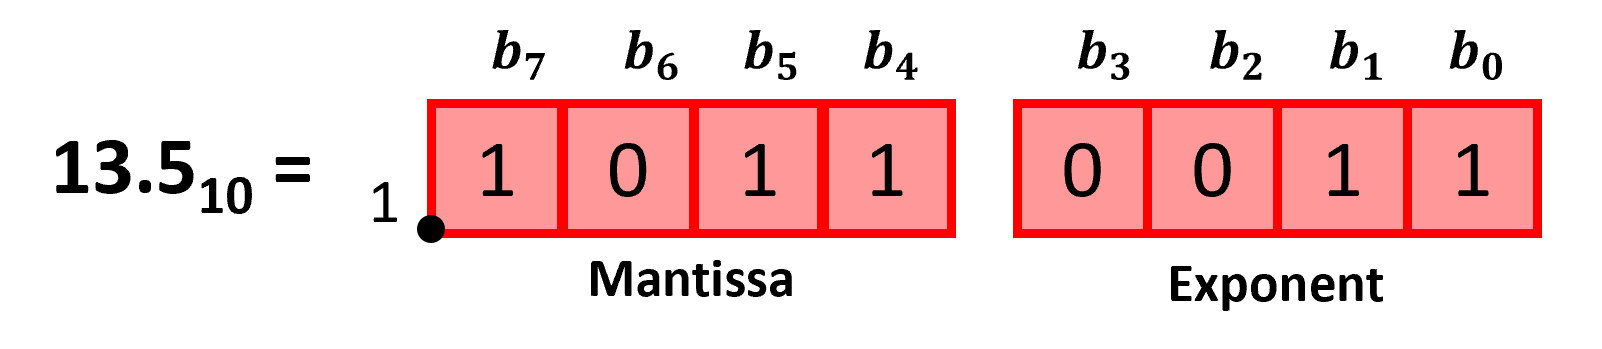
\includegraphics[width= 0.8\textwidth]{./doc/Figures/FloatFloat2.png}
    \caption{Representation of number 13.5 with floating-point format using only 1 byte (8 bits).}
    \label{fig:FloatFloat}
\end{figure}

Since the integer part of the mantissa is always 1, we only need to encode the fractional part.
Given a binary floating point representation with these 8 bits ($b_7, \ldots, b_0$) 
and noticing that $b_3 = 0$ encodes a positive exponent and $b_3 = 1$ a negative exponent, 
the decimal number is obtained by:
$$
   x = m \ 2^e, \quad m =  b_7 \ 2^{-1}  + b_6 \ 2^{-2} + b_5 \ 2^{-3} + b_4 \ 2^{-4}, \quad 
    e =  (-1)^{b_3} (  b_2 \ 2^{2} + b_1 \ 2^{1} + b_0 \ 2^{0} ) 
$$

The maximum value allowed with this representation is: 
$$
   \texttt{1111 0111} = 1.9375 \times 2^{7}
$$   
and the smallest number is: 
$$
   \texttt{0000 1111} =  2^{-7}.
$$ 
In this representation, the distance between the maximum number and its closest number is $2^3$
and the distance between the minimum number and its closest number is $ 2^{-11}$. Hence, in a 
much bigger range we manage variable distances between reals, extremely shorts near 0 and really big 
for bigger values. 





To conclude, for the same number of bits, fixed-point numbers are equal-spaced along 
the whole range but with a smaller range ($31.875$ vs $ 1.9375 \times 2^{7}$).
The distance among real numbers in the fixed-point representation is constant ($0.125$ in our example). 
However, in the floating-point representation, the distance among real numbers 
changes from extremely short values to very big distances ($2^{-11}$ to $ 2^{7}$) depending on the exponent of the real number. 
never forget that the total amount of real numbers in fixed point or floating point 
representation is exactly the same but their distribution and range are different.


\begin{IN}
    \begin{enumerate}
        \item Fixed-point format has constant distance among all representable real numbers and a small range. 
        \item Floating-point format has variable distance among all representable real numbers with a huge range.  
    \end{enumerate}
\end{IN}


In the following section the standard IEEE 754, which is used in all computers, is 
explained in detail to understand how real numbers are stored in floating point representation.


%I change this part

%In order to compare with floating-point representation
%let's consider a mini-float of same size, 8 bits.
%In this case 4 bits are reserved for the exponent (1 for its sign and 3 for its value) 
%and 4 bits for the mantissa. 
%Once again no negative values are encoded.
%
%Since the integer part of the mantissa is always a 1 we just need to encode the fractional part.
%Given a binary floating point representation with these 8 bits ($b_7, \ldots, b_0$), 
%the decimal number is obtained by:
%$$
%x = m \ 2^e, \quad m =  b_7 \ 2^{-1}  + b_6 \ 2^{-2} + b_5 \ 2^{-3} + b_4 \ 2^{-3}, \quad 
%e =  \pm (  b_2 \ 2^{2} + b_1 \ 2^{1} + b_0 \ 2^{0} ) 
%$$
%The maximum value with this representation is: 
%$$
%\texttt{1111 1111} = 15 \times 2^{7}
%$$   
%and the smallest number is: 
%$$
%\texttt{0001 0111} =  2^{-7}.
%$$ 
%The distance between the maximum number and its closest  number is:  $  2^{7}$
%and the distance between the minimum number and its closest number is:  
%$ 2^{-7}.$



%%%%RESTOS

%These are not used in numerical calculations where simple precision (4 bytes) 
%is the smallest precision used. 
%However, it needs from the same amount of memory space 
%as the previous example so it can be a good comparison to understand the concept. 

%Do not worry if the notation is not clear right now, it is explained later for the 4-bytes precision, 
%which is similar. 

% and an exponent bias of +7 
%(these concepts are broaden in this section). 
%This representation allows a range between $r\in (-480 = 1 1111 111_2, 480 = \texttt{0 1111 111}_2)$ 
%and 


% $0.0078125_{10} =_2$. 
%We are not discussing now if the number $0 0000 000_2$ is reserved for the $0$ 
%or the number $\texttt{0 1111 111}$ or $\texttt{1 1111 111}$ are reserved for $\pm\infty$ 
%since this is just an example of the capabilities of floating-point representation. 

%In order to compare with floating-point representation,
%let's consider a mini-float of 8 bits with the same memory size that 
%the above fixed point representation. 
%Consider a mini-float with
%4 bits for the exponent (1 for its sign and 3 for its value) and 4  bits for the mantissa.
%Giving a binary floating point representation with 8 bits ($b_7, \ldots, b_0$), 
%the decimal number is obtained by: 


%There are two main ways to represent real numbers in computers: 
%\begin{itemize}
%    \item Fixed-point representation. 
%The real number is represented by its integer part and its decimal part (e.g. \texttt{55.88}). 
%    \item Floating-point representation. 
% The real number is represented by its mantissa and its exponent  (e.g. \texttt{0.5588e02}).
%\end{itemize} 

%     Fixed-point format actually could represent larger numbers or smaller numbers,
%     but it has a static range, which means that the choose is done when designing the code, 
%     later you can only use that range, 
%     either big or small numbers. 
%     Luckily, floating-point format has dynamic range, 
%     which means that once designed the format it can handle 
%     at the same time large and tiny numbers just varying the exponent. 




    %--------------------------------------------------------------------------------------------------------------------------------------
    \section{Floating-point representation in IEEE 754}


Before delving into the particularities of the representation in the standard IEEE 754 a summary of the main properties is presented here. 
\begin{enumerate}
    \item Similarly to the binary normalized scientific notation, the binary point is located immediately after the first binary digit of the mantissa which is always a 1 (normalized range) and it is not explicitly stored. 
    \item The leftmost digit encodes the sign of the number: 1 for negative number, 0 for positive.
    \item The rightmost digits encode the mantissa. 
    \item Between sign bit and mantissa, the exponent is encoded with an offset-binary representation (using an exponent bias).
\end{enumerate} 

Notice from the table \ref{tab:properties} that the actual bits used in the mantissa is always the number of mantissa bits + 1. 
This is due to an implicit 1 in the left part of binary point, since it is always a 1, is not explicitly stored. 
Hence, the binary mantissa of the example $-110.3125$ is actually $1.10111001010...$ while only the right part of the binary point is stored.
There is one number that can not be written with an implicit 1 in standard scientific notation; 0. 
This is one of the IEEE exceptions that are treated in section \ref{sec:exceptions}. 

The table also shows the range of representable numbers, the minimum and maximum value allowed for each standard format. 

Finally, the information we are usually more interested in; the decimal precision for each format, which is the number of reliable decimal digits. Consider that $log_2(10)\approx 3.32 $ binary digits are needed in order to represent one single decimal digit. 

For example, in single precision the mantissa counts on 24 binary digits (23 explicitly stored and 1 implicit) so: $24/3.32 = 7.2$. 
Enough precision to have 7 decimal digits reliably represented. 
Notice this does not mean that the first 7 digits of the representation equals the expected value, it means that the relative error between both numbers is around $1e-7$. 
Just consider the number $1.3_{10}$, in the standard IEEE 754 in single precision this value is stored as 
$$
\texttt{0 01111111 01001100110011001100110}_2 = 1.2999999523162841796875_{10}
$$
which means that the error caused by the conversion is $-4.76837158203125E-8$ while only the first digit is the same.

\newpage
\begin{figure}
    \centering
    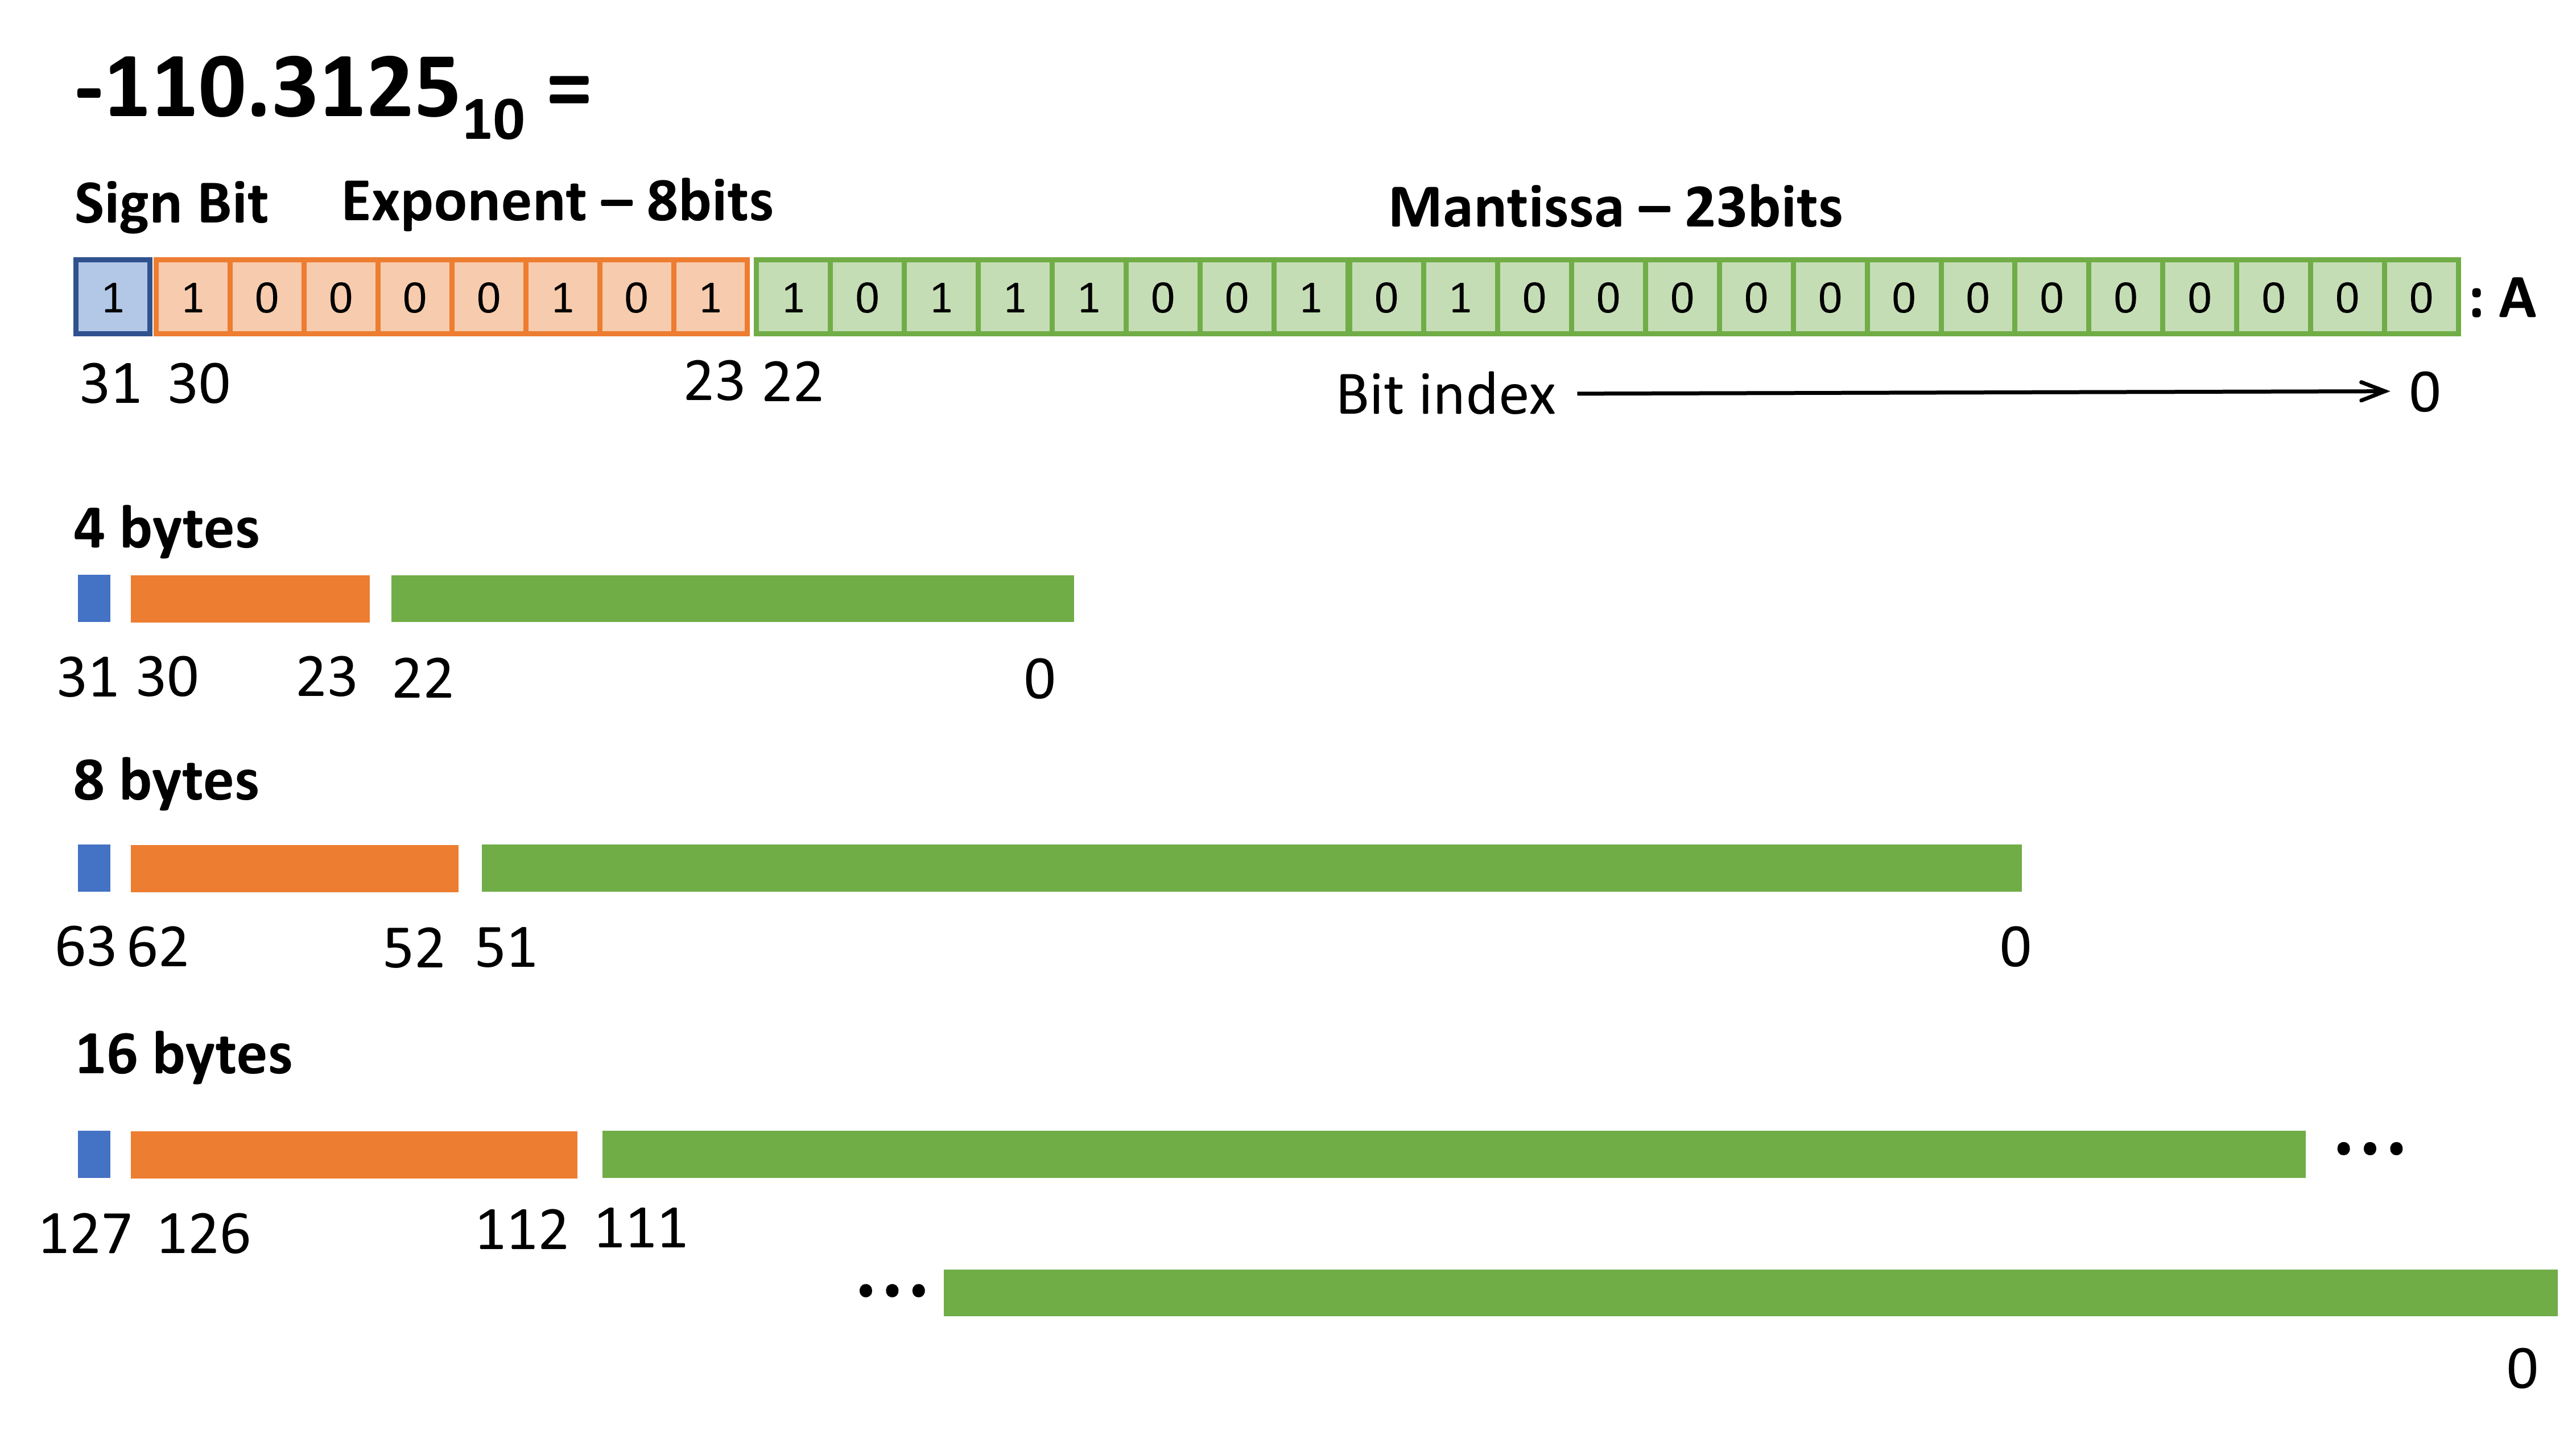
\includegraphics[width= \textwidth]{./doc/Figures/ParametersIEEE.png}
    \caption{Main formats in the standard IEEE 754: single, double and quadruple precision with a visual example in single precision.}
    \label{fig:ParametersIEEE}
\end{figure}
%\begin{table}[H]
%    \centering
%    \begin{tabular}{| r | c | c | c | c | c | }
%        
%        \hline
%        Name & Sign &  \begin{tabular}{@{}c@{}}Exp\\  (r) \end{tabular} &  \begin{tabular}{@{}c@{}}Mantissa\\(p) \end{tabular} & \begin{tabular}{@{}c@{}}Exp. Bias\\  (B) \end{tabular}  & \begin{tabular}{@{}c@{}}Actual Bits\\  mantissa\end{tabular}  \\ \hline
%        
%        \begin{tabular}{@{}c@{}}Single precision \\ (binary32) \end{tabular}      & 1 & 8  & 23    & 127   & 24 \\ \hline
%        
%        \begin{tabular}{@{}c@{}}Double precision \\ (binary64) \end{tabular}    & 1 & 11 & 52    & 1023  & 53   \\  \hline
%        
%        \begin{tabular}{@{}c@{}} Quadruple precision\\(binary128) \end{tabular}   & 1 & 15 & 112   & 16383 & 113   \\ \hline
%        
%    \end{tabular}                                                       
%    %\caption{Main properties of the different precisions covered by the IEEE 754 standard.}
%    %\label{tab:properties}
%\end{table}
%\vspace{-1cm}
%\begin{table}[H]
%    \centering
%    \begin{tabular}{| r | c | c | c |}
%        
%        \hline
%        Name  & \begin{tabular}{@{}c@{}}Normalized \\ range \end{tabular} & \begin{tabular}{@{}c@{}}Approximate\\decimal range\end{tabular} & Precision \\ \hline
%        
%        \begin{tabular}{@{}c@{}}Single precision \\ (binary32) \end{tabular}      &  \begin{tabular}{@{}c@{}}$\pm2^{-126}$ to \\$\pm2^{127+1}$  \end{tabular}    & \begin{tabular}{@{}c@{}}$\pm1.18\cdot10^{ -38}$ to \\ $\pm3.4\cdot10^{38}$ \end{tabular}     & \sim 7 digits  \\ \hline
%        
%        \begin{tabular}{@{}c@{}}Double precision \\ (binary64) \end{tabular}    &  \begin{tabular}{@{}c@{}}  $\pm2^{-1022}$ to\\  $\pm2^{1023+1}$\end{tabular}  & \begin{tabular}{@{}c@{}} $\pm2.23\cdot10^{ -308}$ to \\ $\pm1.80\cdot10^{308}$ \end{tabular} & \sim 15 digits        \\  \hline
%        
%        \begin{tabular}{@{}c@{}} Quadruple precision\\(binary128) \end{tabular}   &  \begin{tabular}{@{}c@{}}  $\pm2^{-16382}$ to\\  $\pm2^{16383+1}$\end{tabular}   & \begin{tabular}{@{}c@{}} $\pm3.3621\cdot 10^{-4932}$ to \\ $\pm1.1897\cdot10^{4932}$ \end{tabular}  & \sim 19 digits          \\ \hline
%        
%    \end{tabular}                                                       
%    \caption{Main properties of the different precisions covered by the IEEE 754 standard.}
%    \label{tab:properties}
%\end{table}

\begin{table}[H]
    \centering
    \begin{tabular}{| r | c | c | c | c | c | }
        
        \hline
        Name & Sign &  \begin{tabular}{@{}c@{}}Exp\\  (r) \end{tabular} &  \begin{tabular}{@{}c@{}}Mantissa\\(p) \end{tabular} & \begin{tabular}{@{}c@{}}Exp. Bias\\  (B) \end{tabular}  & \begin{tabular}{@{}c@{}}Actual Bits\\  mantissa\end{tabular}  \\ \hline
        
        Single precision       & 1 & 8  & 23    & 127   & 24 \\ \hline
        
        Double precision    & 1 & 11 & 52    & 1023  & 53   \\  \hline
        
         Quadruple precision   & 1 & 15 & 112   & 16383 & 113   \\ \hline
        
    \end{tabular}                                                       
    %\caption{Main properties of the different precisions covered by the IEEE 754 standard.}
    %\label{tab:properties}
\end{table}
\begin{table}[H]
    \centering
    \begin{tabular}{| r | c | c | c |}
        
        \hline
        Name  & \begin{tabular}{@{}c@{}}Normalized \\ range \end{tabular} & \begin{tabular}{@{}c@{}}Approximate\\decimal range\end{tabular} & Precision \\ \hline
        
        \begin{tabular}{@{}c@{}}Single precision \\ (binary32) \end{tabular}      &  \begin{tabular}{@{}c@{}}$\pm2^{-126}$ to \\$\pm2^{127+1}$  \end{tabular}    & \begin{tabular}{@{}c@{}}$\pm1.18\cdot10^{ -38}$ to \\ $\pm3.4\cdot10^{38}$ \end{tabular}     & \sim 7 digits  \\ \hline
        
        \begin{tabular}{@{}c@{}}Double precision \\ (binary64) \end{tabular}    &  \begin{tabular}{@{}c@{}}  $\pm2^{-1022}$ to\\  $\pm2^{1023+1}$\end{tabular}  & \begin{tabular}{@{}c@{}} $\pm2.23\cdot10^{ -308}$ to \\ $\pm1.80\cdot10^{308}$ \end{tabular} & \sim 15 digits        \\  \hline
        
        \begin{tabular}{@{}c@{}} Quadruple precision\\(binary128) \end{tabular}   &  \begin{tabular}{@{}c@{}}  $\pm2^{-16382}$ to\\  $\pm2^{16383+1}$\end{tabular}   & \begin{tabular}{@{}c@{}} $\pm3.3621\cdot 10^{-4932}$ to \\ $\pm1.1897\cdot10^{4932}$ \end{tabular}  & \sim 19 digits          \\ \hline
        
    \end{tabular}                                                       
    \caption{Main properties of the different precisions covered by the IEEE 754 standard.}
    \label{tab:properties}
\end{table}








%RESTOS

%\newpage
%%\begin{figure}[h]
%\begin{sidewaysfigure}
%%    %\begin{flushleft}
%%    \centering
%%    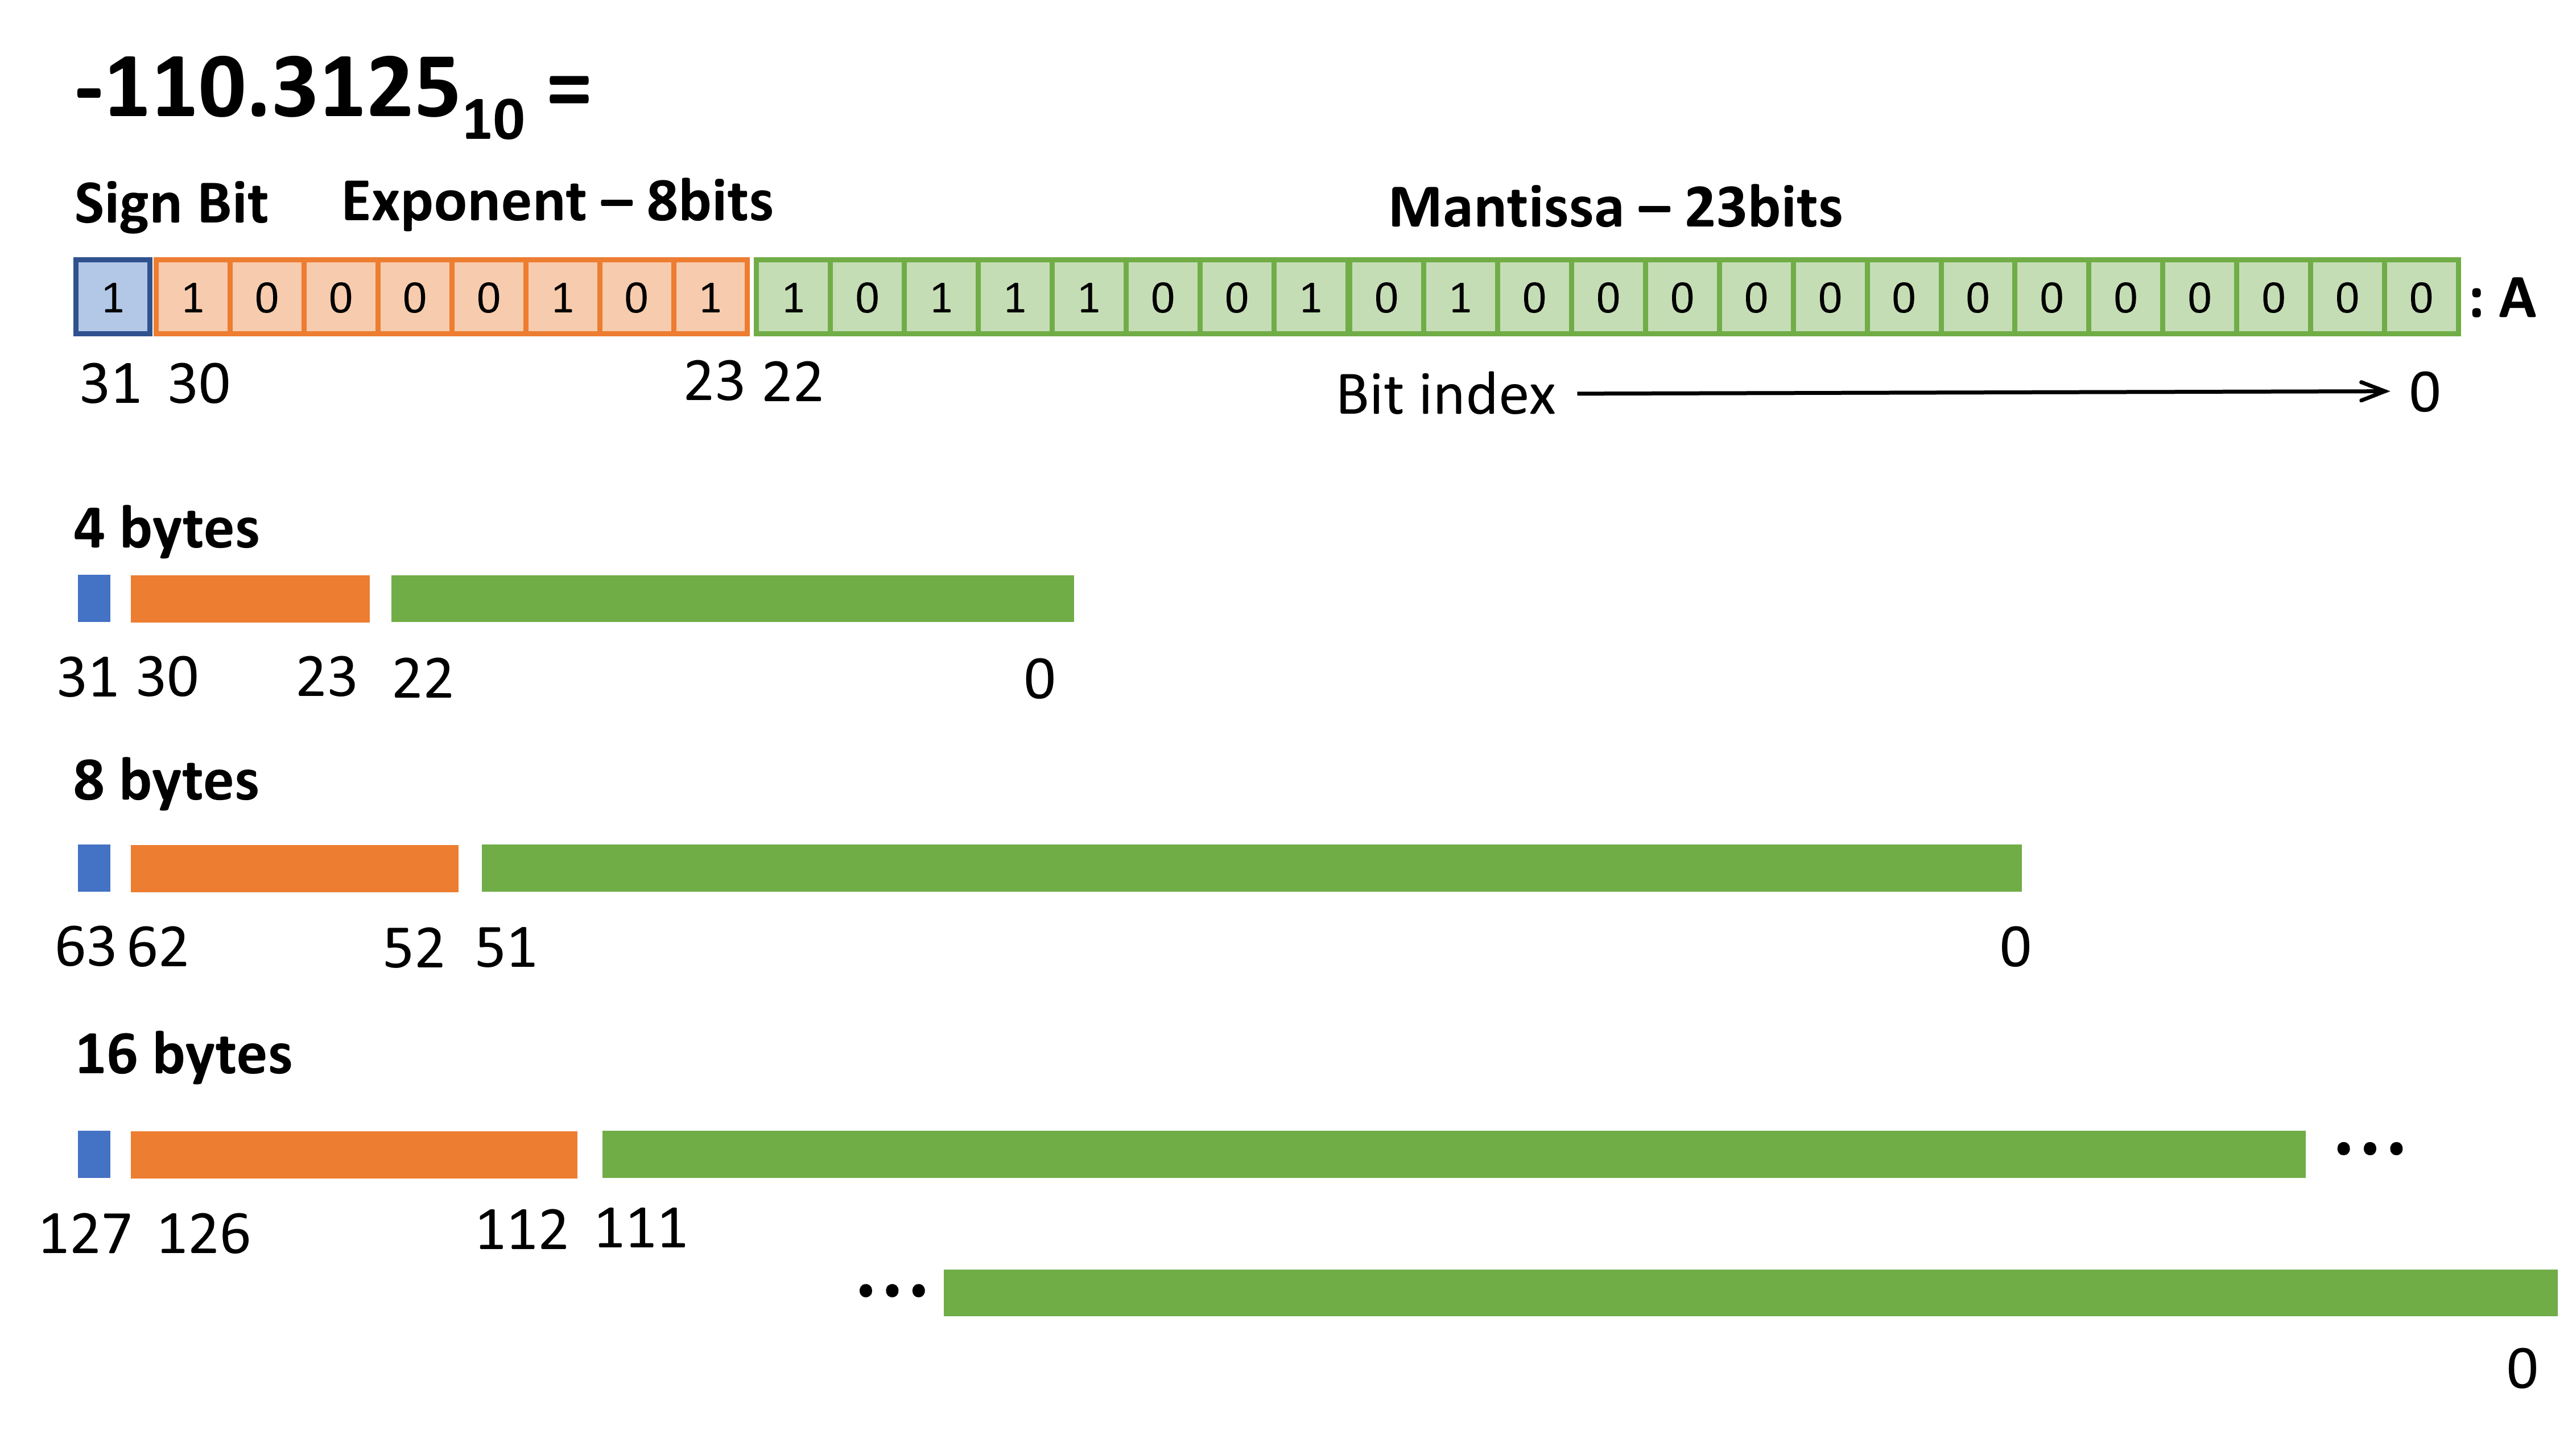
\includegraphics[width= \textwidth]{./doc/Figures/ParametersIEEE.png}
%%    \caption{Main formats in the standard IEEE 754: single, double and quadruple precision with an example in single precision.}
%%    \label{fig:ParametersIEEE}
%%    %\end{flushleft}
%    \begin{table}[H]
%        %\begin{flushright}
%        %\begin{turn}{90}
%        \begin{tabular}{| r | c | c | c | c | c | c | c | c |}
%            
%            \hline
%            Name & Sign & Exp. & Mantissa & Exp. Bias & \begin{tabular}{@{}c@{}}Bits\\  precision\end{tabular}  & \begin{tabular}{@{}c@{}}Normalized \\ range \end{tabular} & \begin{tabular}{@{}c@{}}Approximate\\decimal\end{tabular} & Precision \\ \hline
%            
%            \begin{tabular}{@{}c@{}}Single precision \\ (binary32) \end{tabular}      & 1 & 8  & 23    & +127   & 24 & \begin{tabular}{@{}c@{}}$\pm2^{-126}$ to \\$\pm2^{127+1}$  \end{tabular}    & \begin{tabular}{@{}c@{}}$\pm1.18\cdot10^{ −38}$ to \\ $\pm3.4\cdot10^{38}$ \end{tabular}     & \sim 7.2 digits  \\ \hline
%            
%            \begin{tabular}{@{}c@{}}Double precision \\ (binary64) \end{tabular}    & 1 & 11 & 52    & +1023  & 53 & \begin{tabular}{@{}c@{}}  $\pm2^{-1022}$ to\\  $\pm2^{1023+1}$\end{tabular}  & \begin{tabular}{@{}c@{}} $\pm2.23\cdot10^{ −308}$ to \\ $\pm1.80\cdot10^{308}$ \end{tabular} & \sim 15.9 digits        \\  \hline
%            
%            \begin{tabular}{@{}c@{}} Quadruple precision\\(binary128) \end{tabular}   & 1 & 15 & 112   & +16383 & 113 & \begin{tabular}{@{}c@{}}  $\pm2^{-16382}$ to\\  $\pm2^{16383+1}$\end{tabular}   & \begin{tabular}{@{}c@{}} $\pm3.3621\cdot 10^{-4932}$ to \\ $\pm1.1897\cdot10^{4932}$ \end{tabular}  & \sim 19.2 digits          \\ \hline
%            
%        \end{tabular}                                                       
%        %\end{turn}
%        \caption{Main properties of the different precisions covered by the IEEE 754 standard.}
%        \label{tab:properties}
%        %\end{flushright}
%    \end{table}
%\end{sidewaysfigure}
%%\end{figure}








    %--------------------------------------------------------------------------------------------------------------------------------------
    \newpage 
    \FloatBarrier
    \section{Distance between floating-point real numbers} \label{sec:roundoff}


        %-------------------------------------------------------------------------------------------------------------------------------------- 
        \subsection{Floating-point distribution in the numbers line}

In this section we delve into the relation between the amount of bits reserved to store exponent-mantissa and 
the density of floating-point values in the numbers line. 
Let's consider a vastly simplified format of only 4 bits: $2$ binary digits for the mantissa $p = 2$ (using an implicit 1) and 
$2$ digits for the exponent (four available exponents: $-1, 0, 1, 2$). In addition, not sign bit is considered (see Figure \ref{fig:miniminifloat}).

\begin{minipage}{\textwidth}
    \begin{minipage}{0.3\textwidth}
        \centering
        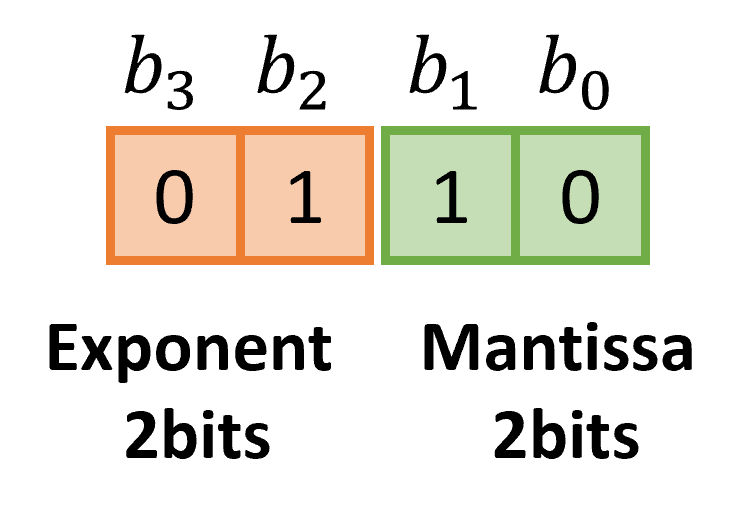
\includegraphics[width= \textwidth]{./doc/Figures/miniminifloat.png}
        \captionof{figure}{Simplified floating-point representation with only 4 bits.}
        \label{fig:miniminifloat}
    \end{minipage}
    \hfill
    \begin{minipage}{0.68\textwidth}
        \centering
        \begin{tabular}{| c | c | c | c | c | }
            \hline
            Mantissa/Exponent   & $-1$ & $0$  & $1$  &   $2$  \\ \hline
            1.00                & $0.5$ & $1$  & $2$  &   $4$  \\ \hline
            1.01                & $0.625$ & $1.25$  & $2.5$  &   $5$  \\ \hline
            1.10                & $0.75$ & $1.5$  & $3$  &   $6$  \\ \hline
            1.11                & $0.875$ & $1.75$  & $3.5$  &   $7$  \\ \hline
        \end{tabular}
        \captionof{table}{Possible decimal values covered by the example system treated.}
        \label{tab:PossibleValues}
    \end{minipage}
\end{minipage}

A general floating-point number in this system is written (see \cite{articleIEEE}): 
$$
1.dd \times 2^{e}    \quad \textrm{with}\quad e \in \mathbb{Z}, e\in\left[-1, 2\right] 
$$ 
A maximum of $2^4 = 16$ values can be represented with this system. 
The possible values, those reals that has exact representation in this system,
are written in the table \ref{tab:PossibleValues} and
plotted in the numbers line of the Figure \ref{fig:DensityNumbers}. 

\begin{figure}[h]
    \centering
    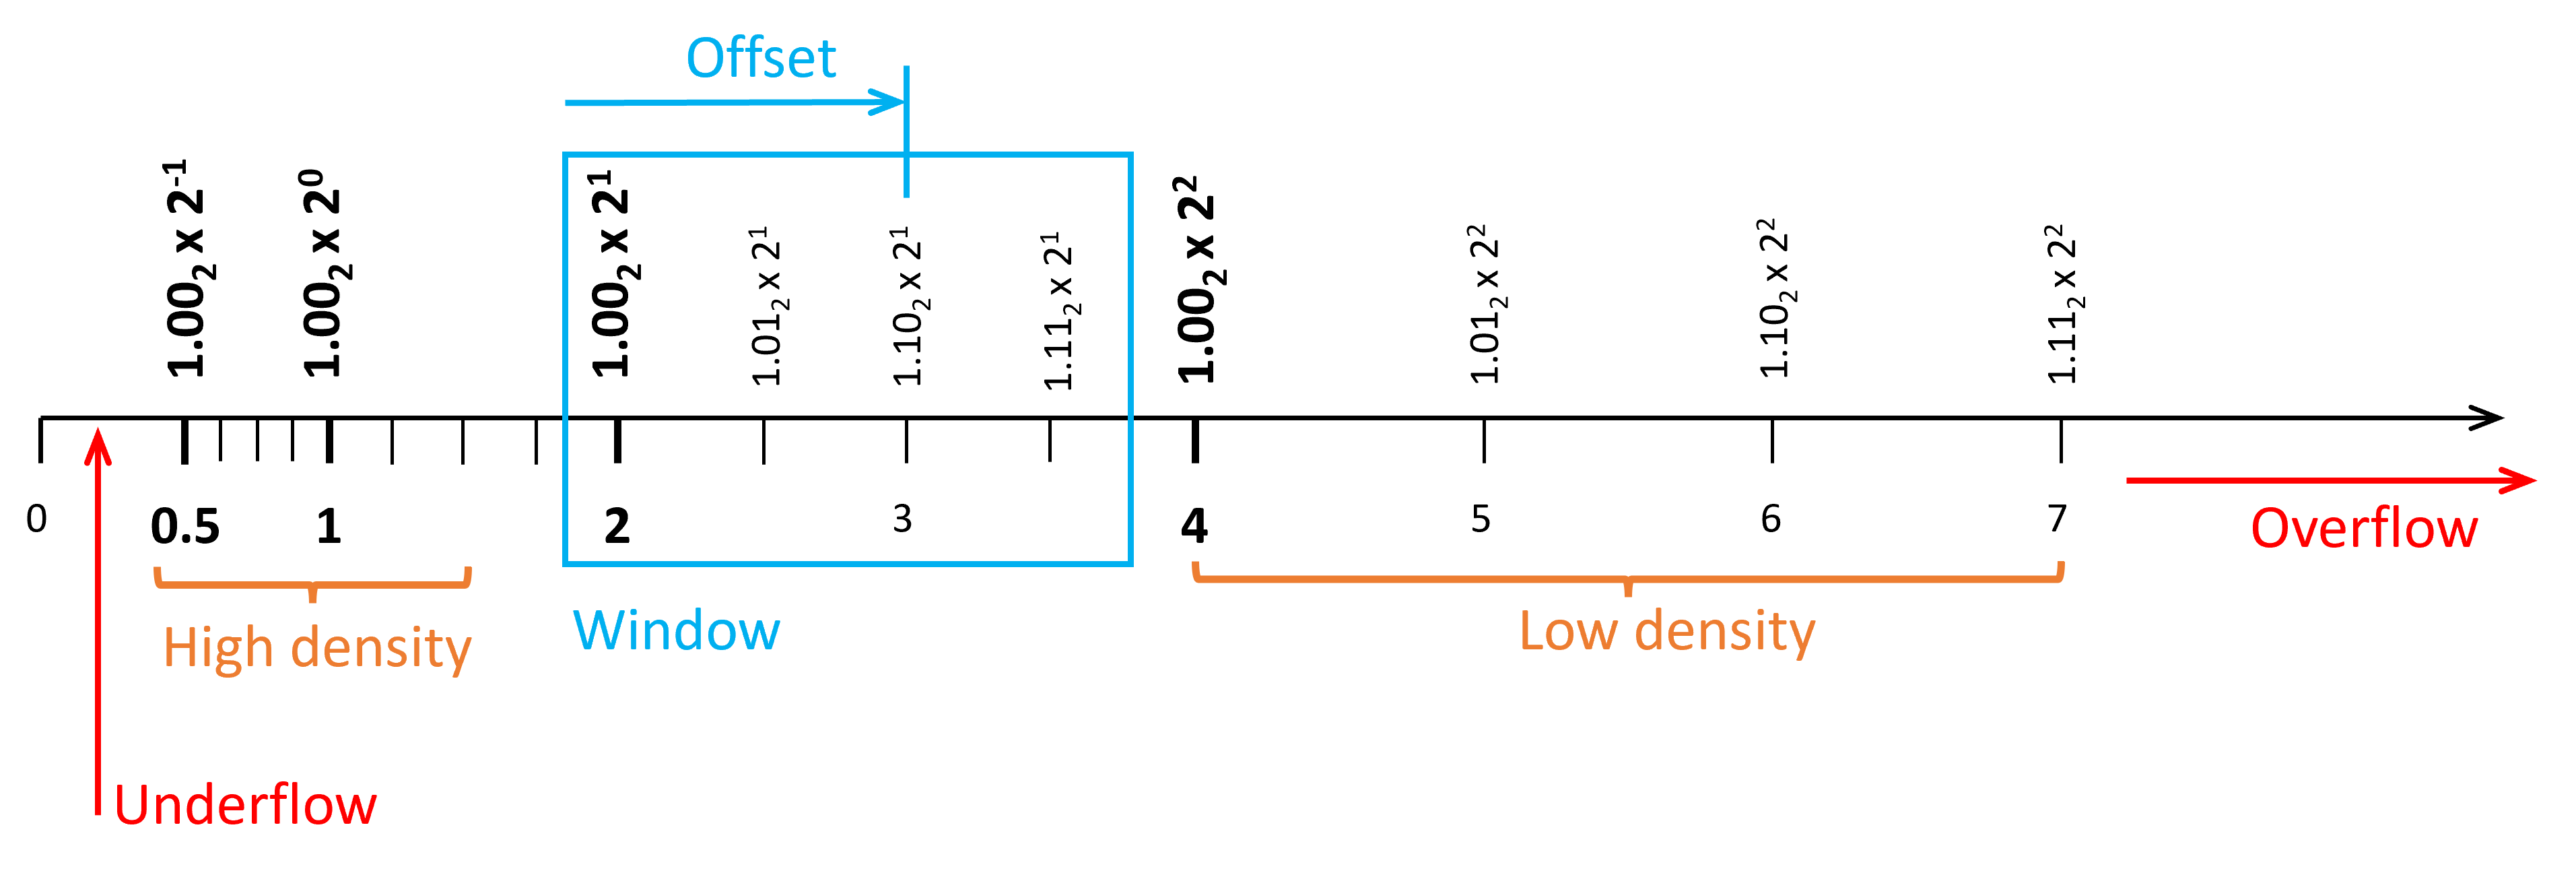
\includegraphics[width= \textwidth]{./doc/Figures/DensityNumbers.png}
    \caption{Representation of the possible values covered by the example system treated.}
    \label{fig:DensityNumbers}
\end{figure}




\FloatBarrier
Think of the exponent as a window between two values 
and the mantissa as the offset of every number inside that window (see \cite{VisExpl}).
In the decimal system a window is limited by two consecutive powers-of-ten: [0.1,1], [1,10], [10,100], etc. 
In binary each window is bounded by powers-of-two: [0.5,1], [1,2], [2,4], etc. 

The exponent of a number fixes its window. Then, 
every window is equidistantly divided according to the number of bits used for the mantissa. 
Both the least significant bit in the mantissa and the exponent tell us the constant distance between values in that window. 

Notice that from one window to the next the number of divisions is the same but the length of the window is twice the previous.
Hence, the resolution in that window is lower and the programmer is loosing capacity to represent numbers. 
Said in other words, the density of floating-point values near the zero is bigger than 
the density of values with growing values. 





%-----------------------------------
It is difficult to represent the density of representable numbers in the numbers line for IEEE 754 standard formats.
However, the behaviour is exactly the same, but with much more values.
Consider a single precision mantissa. 
We count on 23 binary digits to divide every window: $2^{23} = 8688608$ possible values. 

In the window $\left[1,2\right]$ (exponent $0$) the resolution is:
$$
\frac{\left(2-1\right)}{2^{23}} \simeq 0.000000119
$$ 
while in the window $\left[32768=2^{15},65536=2^{16}\right]$ the resolution is:
$$
\frac{\left(65536-32768\right)}{2^{23}} \simeq 0.003906
$$
To conclude, the density of numbers that are exactly represented in IEEE 754 decreases 
when we move away from 0 on the numbers line. 
%-----------------------------------





%RESTOS
%\begin{figure}[H]
%    \centering
%    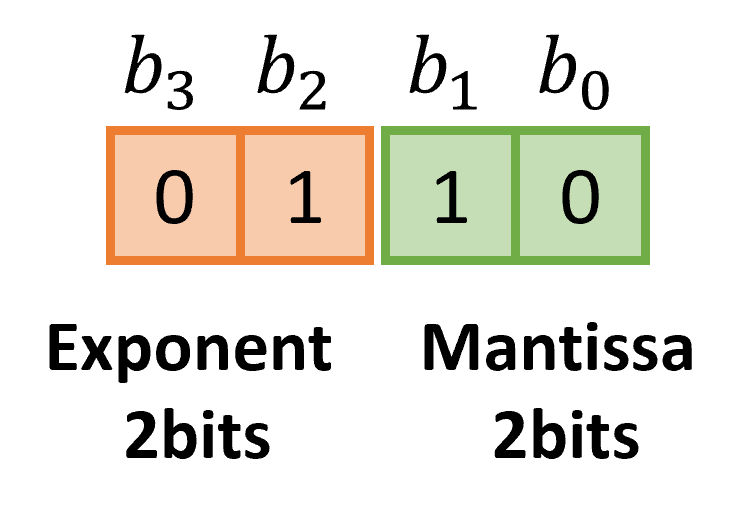
\includegraphics[width= .3\textwidth]{./doc/Figures/miniminifloat.png}
%    \caption{Simplified floating-point representation with only 4 bits.}
%    \label{fig:miniminifloat}
%\end{figure}

%\begin{table}
%    \centering
%    \begin{tabular}{| c | c | c | c | c | }
%        \hline
%        Mantissa/Exponent   & $-1$ & $0$  & $1$  &   $2$  \\ \hline
%        1.00                & $0.5$ & $1$  & $2$  &   $4$  \\ \hline
%        1.01                & $0.625$ & $1.25$  & $2.5$  &   $5$  \\ \hline
%        1.10                & $0.75$ & $1.5$  & $3$  &   $6$  \\ \hline
%        1.11                & $0.875$ & $1.75$  & $3.5$  &   $7$  \\ \hline
%    \end{tabular}
%    \caption{Possible decimal values covered by the example system treated.}
%    \label{tab:PossibleValues}
%\end{table}


        %-------------------------------------------------------------------------------------------------------------------------------------- 
        \subsection{Absolute and relative error}


The question that arises at this point is: Which is the round-off error when using finite precision floating-point reals?

%-----------------------------------
Let's see an example using the 4-bits system explained in the previous section. Imagine that you need to use the constant: 
$$
3.1875_{10} = 11.0011_2 = 1.10011\times 2^1_2
$$
This number does not have exact representation as we can check in Table \ref{tab:PossibleValues}. It will be rounded to the nearest representable number, which is: 
$$
1.10\times2^1_2 = 3_{10}
$$
The round-off error is $3.1875_{10} - 3_{10} = 0.1875_{10} = 0.0011_2$.
 
Notice that the last representable binary place for the number $1.10\times2^1_2$ is $0.01\times2^1 = 0.1_2$ 
so the error made in our approximation can also be expressed as $0.011_2$ units in the last place (\textit{ulps} $= 2^{e-p}$). 
%-----------------------------------



{\Large Absolute Error}

For a given value $z$ and its representation in a floating-point system $z_{fl}$, 
the absolute error made is the distance between them:
$$
E_{abs} = \abs{z - z_{fl}} 
$$
This error can be expressed by the distance itself or using ulp.

The absolute error for our theoretical 4-bits system is plotted in Figure \ref{fig:AbsErrorGraph}.
\begin{figure}[h]
    \centering
    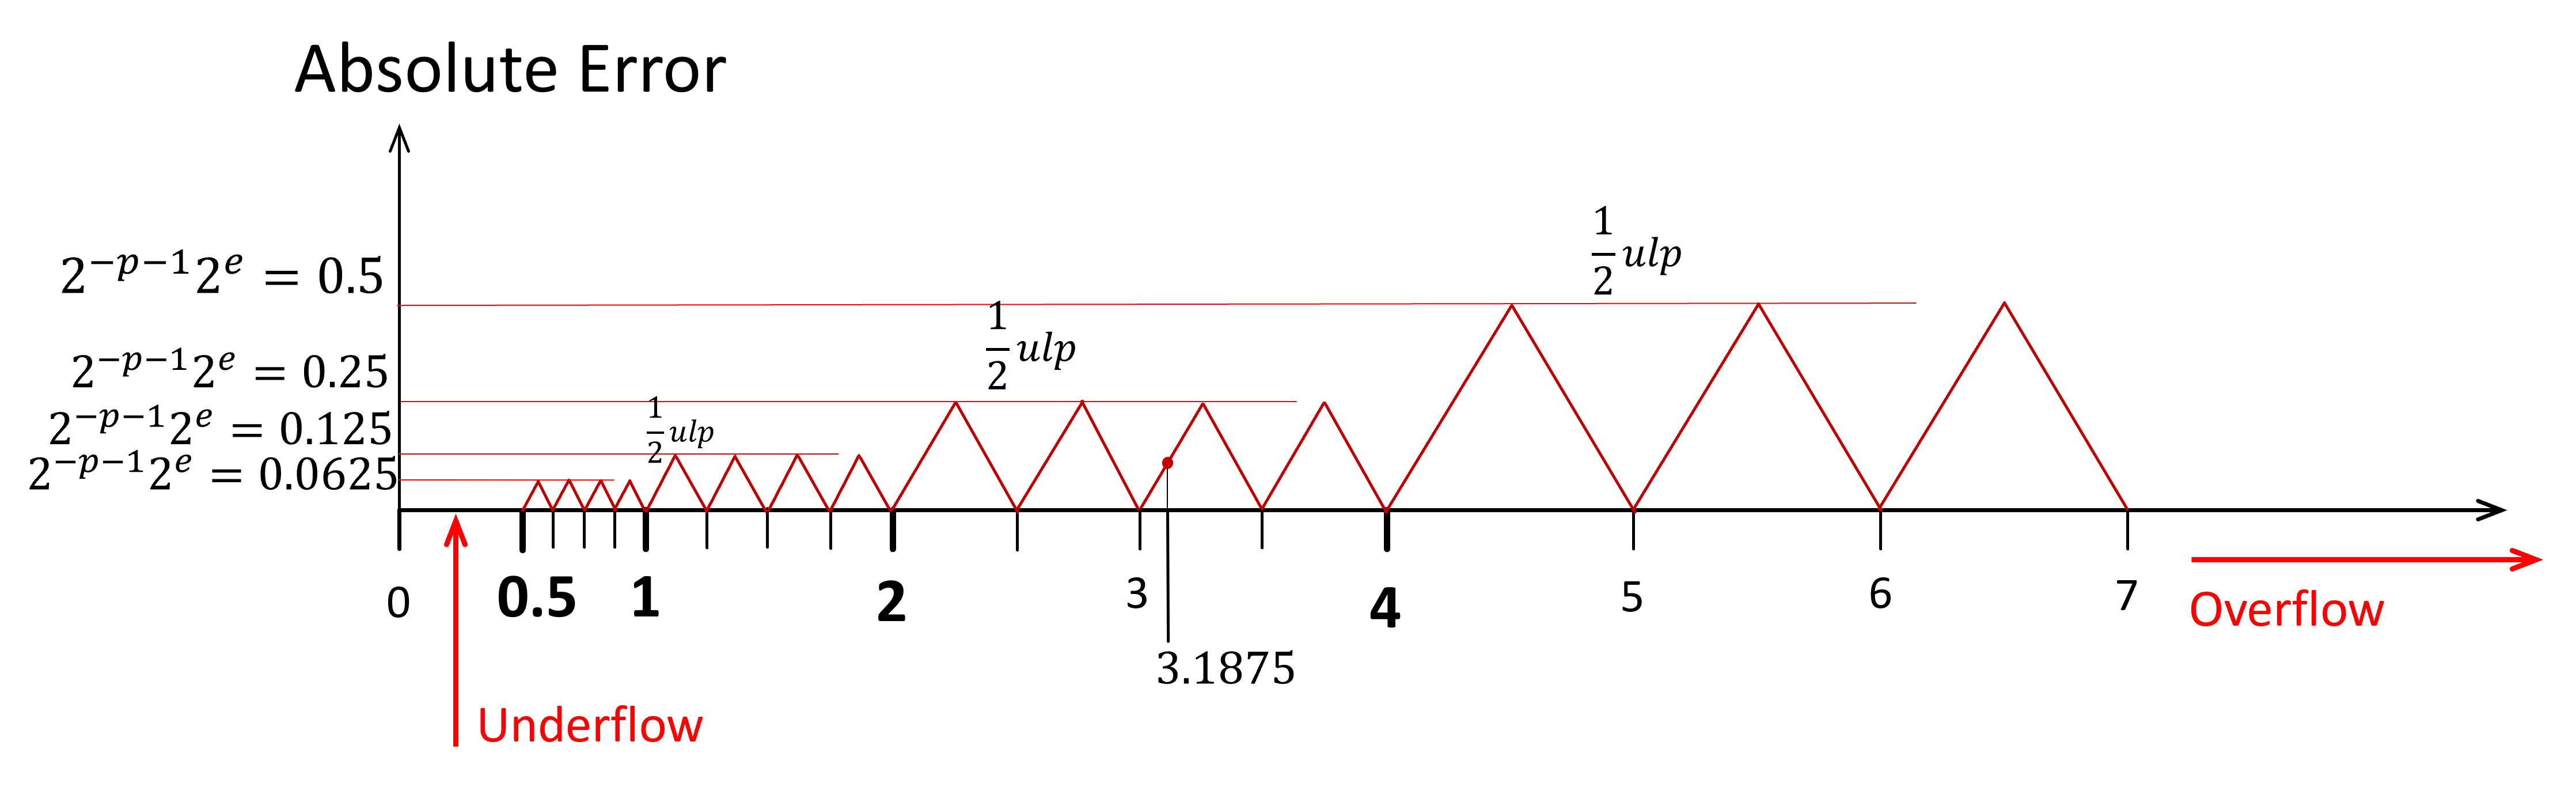
\includegraphics[width= \textwidth]{./doc/Figures/AbsErrorGraph.png}
    \caption{Absolute error made when the reals are approximated by the nearest floating-point value. Notice that reals are attracted by the floating-point values which act as a magnetic grid.}
    \label{fig:AbsErrorGraph}
\end{figure}

Notice that when the exact number is approximated by the nearest floating-point value 
this error is always \textbf{bounded} by half ulp ($0.5_{10}$ ulp $= 0.1_2$ ulp). 
Expressed with ulp seems that this bound is small but remember that the concept \textit{ulp} depends both on 
the binary \textbf{digits of the mantissa} and the \textbf{exponent of the represented number}.
Half ulp is much more important if we are representing a number around $2^{24}$ than a number near $2^1$.





{\Large Relative Error}


Another way to measure the error made in the representation is using the relative error:
$$
E_{rel} = \abs{\frac{z - z_{fl}}{z}} = \abs{1 - \frac{z_{fl}}{z}}
$$
Now, the difference between exact and approximated number is divided by the exact value so
the error does not grow while moving along the numbers line, 
it remains bounded for the whole range. 

The relative error for our theoretical 4-bits system is plotted in Figure \ref{fig:RelErrorGraph}.
\begin{figure}[h]
    \centering
    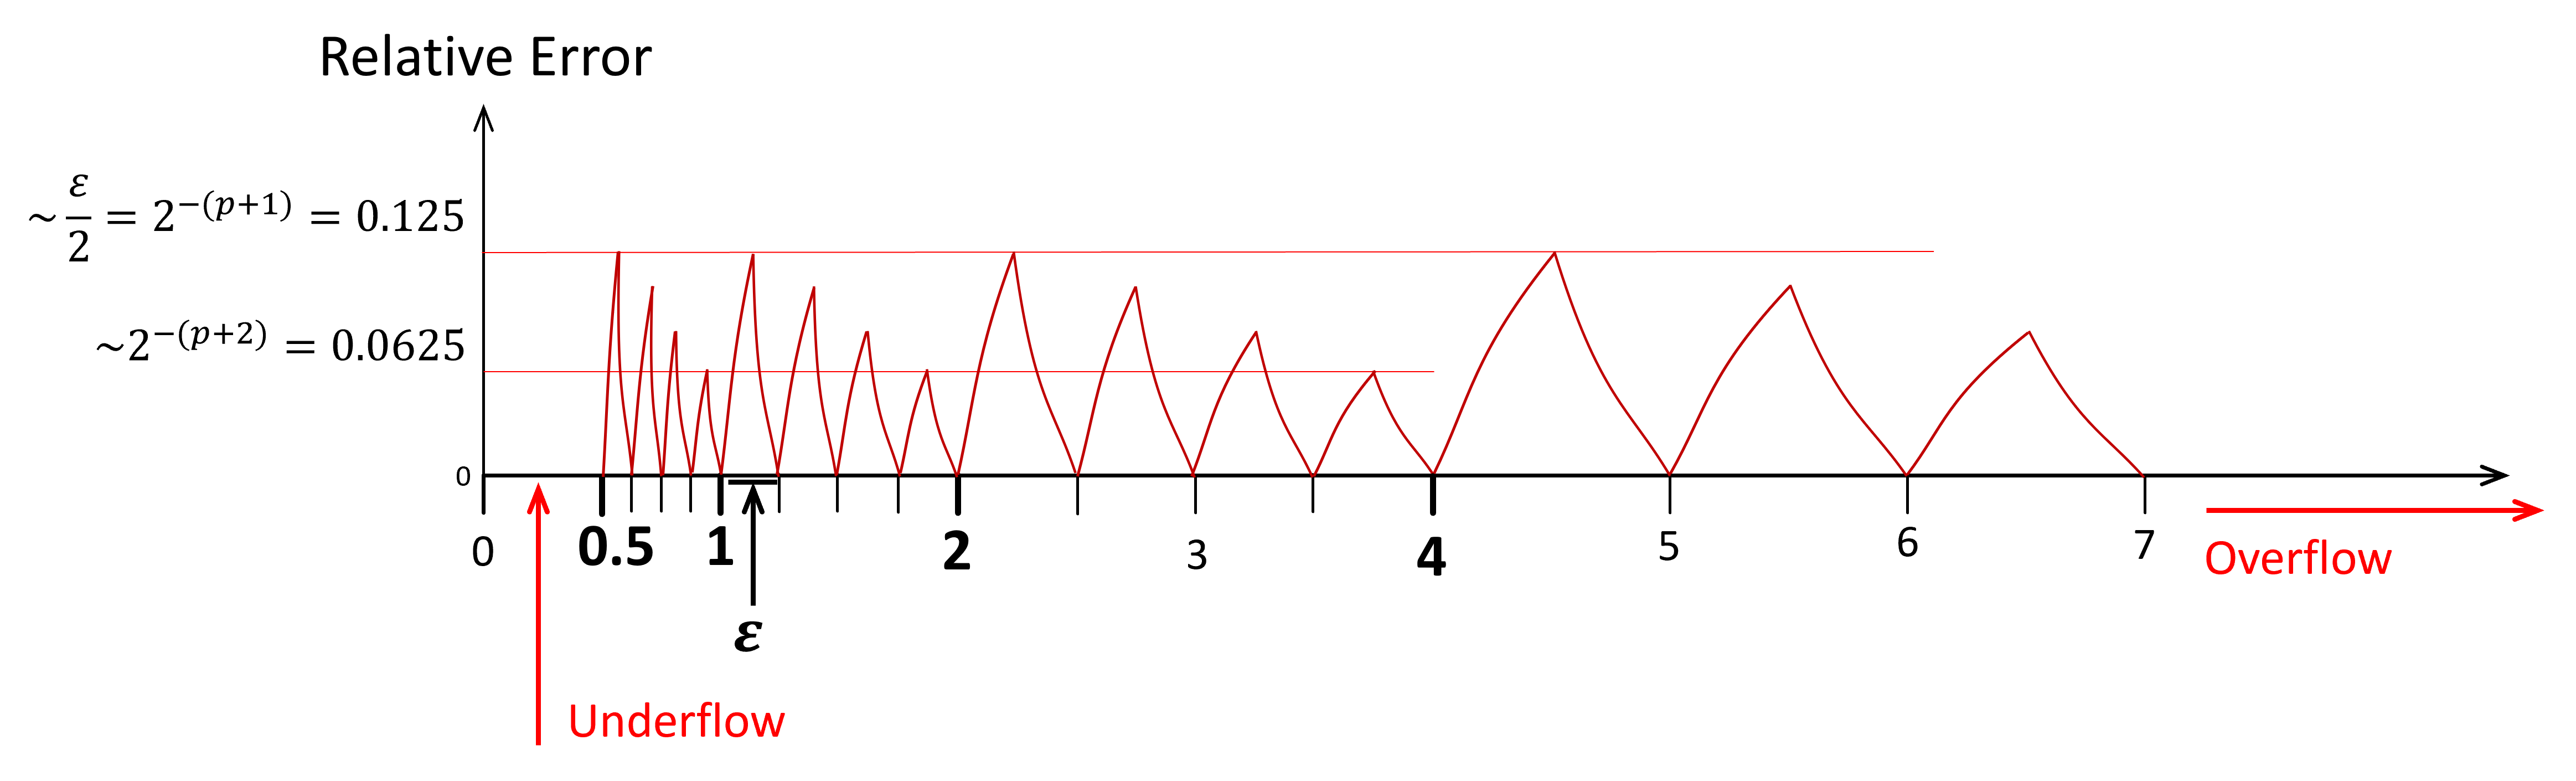
\includegraphics[width= \textwidth]{./doc/Figures/RelErrorGraph.png}
    \caption{Relative error made when the reals are approximated by the nearest floating-point value.}
    \label{fig:RelErrorGraph}
\end{figure}

When the exact number is approximated by the nearest floating-point value we can also find an expression 
for the bounds of this error. Let's find the relative error associated to the maximums of the absolute error made in any window.
For every window (exponent) $z$ varies in the range 
$$
z \in \left[2^e, 2\times 2^e\right)
$$ 
and the maximum absolute error in that window is $\frac{1}{2}\textrm{ulp} = 2^{e-p-1}$.
Then, the maximums of the relative error ranges in:
$$
\left[\frac{2^{e-p-1}}{2^{e+1}},  \frac{2^{e-p-1}}{2^e} \right] = \left[2^{-(p+2)},  2^{-(p+1)} \right]
$$
The highest value of the different peaks happens around the beginning of the window, 
when the value of $z$ is lower (see Figure \ref{fig:RelErrorGraph}). 







This example imitates perfectly what happen with IEEE 754 floating-point formats. Both errors behave in the same way but with different values. 
The table \ref{tab:errors} shows these magnitudes generalised for any binary floating-point format where 
$p$ is the number of digits reserved for the mantissa and $e$ is the exponent of the value $z$ to be represented.
\begin{table}
    \centering
    \begin{tabular}{| c | l | }
        \hline
        \textbf{Definition}       & \textbf{Expression}  \\ \hline %%%%%%
        ulp                       & $2^{e-p} = 0.0000...01 \times 2^e $  \\ \hline
        Absolute error of $z$     & $ \abs{z - z_{fl}} = \abs{z - 1.dddd...\times 2^e} $ \\ \hline   %%%%%%%
        \begin{tabular}{@{}c@{}} Max absolute error   \\    for a given exponent    \end{tabular}    & $ \frac{1}{2} ulp = 2^{e-p-1}$  \\ \hline   %%%%%%%
        Relative error            & $ \abs{\frac{z - z_{fl}}{z}} = \abs{1 - \frac{z_{fl}}{z}} = \abs{\frac{z - 1.dddd...\times 2^e}{z}}$  \\ \hline
        Bounds for relative error   & $\left[2^{-(p+2)}, 2^{-(p+1)} \right]$   \\ \hline     %%%%%%%
    \end{tabular}
    \caption{Main magnitudes that describe the representation of a value $z$ in a floating-point binary format when it is approximated by the nearest floating-point value $z_{fl}$.}
    \label{tab:errors}
\end{table}

When a variable is initialized or a constant value defined, the exact value is approximated by the nearest IEEE 754 number. Then, we have seen that the absolute error is bounded. 
On the contrary, when operating (adding, multiplying, dividing, etc.) with reals, the finite precision result of the operation could be different from the nearest IEEE value to the exact result.
The absolute error, whether expressed in units or with ulps, is usually used to understand the rounding error along the numbers line. However, the relative error is better to analyse calculations.  

\begin{IN}
    \begin{itemize}
        \item The term \textit{ulp} is used to indicate the last representable binary place for a floating point, it depends on the number of mantissa digits and the exponent of the number to be represented: $ulp = 2^{e-p}$. 
        \item The absolute round-off error grows with the exponent but always bounded by $\frac{1}{2} ulp = 2^{e-p-1}$.
        \item The relative round-off error is bounded by a constant value along the numbers line equal to $2^{-(p+1)}$.
    \end{itemize}   
\end{IN} 




%\begin{IN}
%    \begin{itemize}
%        \item Use the absolute error, whether expressed in units or with ulps, to understand the rounding error along the numbers line. 
%        \item Use the relative error to analyse the results of your calculations in the computer.
%    \end{itemize}   
%\end{IN}  



%RESTOS
%which in our example system is:
%$$
%E_{abs} =  \abs{z - 1.dd\times 2^e} = \abs{ \left(  \frac{z}{2^e}  \right) - 1.dd }2^e
%$$

%\begin{table}
%    \centering
%    \begin{tabular}{| c | l | }
%        \hline
%        \textbf{Definition}       & \textbf{Expression}  \\ \hline %%%%%%
%        ulp                       & $2^{e-p} = 0.0000...1 \times 2^e $  \\ \hline
%        Absolute error of $z$     & $ \abs{d.dddd...\times 2^e - z} = \abs{d.dddd...-\frac{z}{2^e}} 2^e $ \\ \hline   %%%%%%%
%        Maximum absolute error    & $\frac{2^{-p}2^e}{2} = \frac{1}{2} ulp$  \\ \hline   %%%%%%%
%        Relative error            & $\abs{\frac{z - d.dddd...\times 2^e}{z}}$  \\ \hline
%        \begin{tabular}{@{}c@{}} Relative error of the   \\    maximum absolute error    \end{tabular}  & 
%        $\left[2^{-(p+2)}, 2^{-(p+1)} \right]$   \\ \hline     %%%%%%%
%    \end{tabular}
%    \caption{Different errors committed when the real number $z$ is approximated by the nearest floating-point value. Remember that here $p$ is the number of bits of the mantissa excluding the implicit 1. }
%    \label{tab:errors}
%\end{table}


        %--------------------------------------------------------------------------------------------------------------------------------------
        \FloatBarrier
        \subsection{Machine epsilon}

The importance of machine epsilon lies in the fact that this magnitude bounds the 
relative error of any number when is rounded to the closest floating-point value. 
Different definitions are used, however, we consider the following: 
it is the smallest number $\epsilon$ such that $1 + \epsilon > 1$. 
In other words, the distance between 1 and the next larger floating point number (see Figure \ref{fig:RelErrorGraph}).

Machine epsilon is then the smallest change we can make to the number 1 and is obtained by adding one to the least significant bit of the mantissa. 
Hence, calling $p$ to the number of significant digits of the mantissa not including the implicit 1 (see Table \ref{tab:eps}):
$$
\epsilon = 2^{-p}
$$ 

\textit{Notice that sometimes $p$ is used for the mantissa digits including the implicit 1 so a slightly different expression of this machine epsilon can be found.}

Formally, when the exact value to be represented is rounded to the nearest floating-point value, 
the relative error is not bounded by $\epsilon$ but $\frac{\epsilon}{2}$ which is called \textit{unit roundoff}:
$$
\frac{\epsilon}{2} = 2^{-p-1}
$$


\begin{table}[H]
    \centering
    \begin{tabular}{| r | c | c | c | }
        
        \hline
        Name  &  Mantissa (p) & $\epsilon$ & $\frac{\epsilon}{2}$  \\ \hline
        
        \begin{tabular}{@{}c@{}}Single precision \\ (binary32) \end{tabular}     &  23    & $\sim 1.19\cdot10^{-7} $   & $\sim 5.96\cdot10^{-8} $ \\ \hline
        
        \begin{tabular}{@{}c@{}}Double precision \\ (binary64) \end{tabular}    &  52    & $\sim 2.22\cdot10^{-16} $  & $\sim 1.11\cdot10^{-16} $   \\  \hline
        
        \begin{tabular}{@{}c@{}} Quadruple precision\\(binary128) \end{tabular}  & 112   & $\sim 1.93\cdot10^{-34}  $  & $\sim 9.63\cdot10^{-35} $   \\ \hline
        
    \end{tabular}                                                       
    \caption{Bounds of the relative error for the different formats covered by the IEEE 754 standard.}
    \label{tab:eps}
\end{table}



It can be concluded from this chapter that the density of numbers that can be represented near 0 is enormous and this density decreases as 
we move away from 0. A scientific programmer can take advantage of this property and normalize the operations to perform. 
For example, consider an ODE solution where the whole equation is dimensionless with all the terms divided by the 
maximum values that the variables are going to reach. The solution varies around 1, where the IEEE 754 floating point 
set is more dense and the absolute error is lower. 




        %--------------------------------------------------------------------------------------------------------------------------------------
        \subsection{Are integer numbers exactly represented in the reals?}


Integer values in the field of reals follow the same treatment as any other real number so they will be exactly represented with the same number of decimal digits. 
Hence, not all the integers contained in the representable range of real numbers have exact representation in this set. 

In the case of single precision for example, at least all the integers with 6 or less significant decimal digits can be converted to a IEEE 754 value without losing precision. 
Some integers with 9 digits can also be converted but more than 9 digits is inevitably related to loss of precision. 

As an example, the following number is exactly stored: 
$$
899565_{10} = \texttt{0 10010010 10110111001111011010000}
$$
but the number $45962178_{10}$ is converted (with an error of $-2$ units) to:
$$
45962176_{10} = \texttt{0 10011000 01011110101010011110000}
$$



%RESTOS
%There are two reasons why a real number you may want to represent in the computer can not be 
%exactly represented and has to be rounded to an IEEE floating-point value. 
%The first and the less common, the number is out of the 
%representable range either for an overflow or an underflow.
%The second; there is not binary representation for that number, maybe its binary translation has infinite number of 
%digits or maybe it has more significant digits than the allowed by the format used (precision, see 
%\cite{articleIEEE}). 


%RESTOS GENERICOS USANDO beta 

%Let's also find bounds for the relative error, for example, the relative error of the maximum absolute error committed in any window. 
%In this case, for every exponent, the 
%real number varies in the range $z \in \left[\beta^e, \beta \beta^e\right)$ while the maximum absolute error is constant 
%$\frac{1}{2}\textrm{ulp}$ so the relative error ranges in: $\left[\frac{\beta}{2}\beta^{-p}, \frac{1}{2}\beta^{-p} \right]$
%
%\begin{IN}
%    Use the absolute error, whether expressed absolutely or with ulps, to understand the rounding error and use the relative error to analyse 
%    the results of calculations in the computer.
%\end{IN}  
%
%For a general number system where $\beta$ is the base of the system, $p$ is the number of digits reserved for the mantissa and $e$ is the 
%exponent, the table \ref{tab:errors} shows the errors and their bounds. Notice that the definition of the ulp is composed by a part that 
%depends number system ($\beta$ and $p$) and another part that depends on the specific exponent that is represented (the window), $e$. 
%
%\begin{table}
%    \centering
%    \begin{tabular}{| c | l | }
%        \hline
%        \textbf{Definition}   & \textbf{Expression }  \\ \hline
%        ulp                & $\beta\beta^{-p}\beta^e = 0.0000...\beta' \textrm{x} \beta^e    \quad     \textrm{with} \quad \beta' = 
%        \frac{\beta}{2} \textrm{digits}$  \\ \hline
%        Absolute error of $z$             & $\abs{d.dddd...\textrm{x} \beta^e - z} = \abs{d.dddd...-\frac{z}{\beta^e}}\beta^e$ \\ \hline
%        Maximum absolute error            & $\left[\left(\frac{\beta}{2}\right)\beta^{-p}\right]\beta^e = \frac{1}{2} ulp$  \\ \hline
%        Relative error                & $\abs{\frac{z - d.dddd...\textrm{x} \beta^e}{z}}$  \\ \hline
%        \begin{tabular}{@{}c@{}} Relative error of the   \\    maximum absolute error    \end{tabular}           & 
%        $\left[\frac{1}{2}\beta^{-p}, \frac{\beta}{2}\beta^{-p} \right]$   \\ \hline
%    \end{tabular}
%    \caption{Different errors committed when the real number $z$ is approximated by the nearest floating-point value.}
%    \label{tab:errors}
%\end{table}
%
%A good way to understand the expressions and behaviour of these errors is to represented them in the same number line shown above, using that 
%representation system. Because of the high density of the representable number in the IEEE-754 system for simple precision, in that case only 
%the boundaries of the errors are represented, while in the simpler case of only 3 significant digits, is possible to show the exact error for 
%every real number (see Figure \ref{fig:AbsErrorGraph}).
%
%For the relative error, take into account that the each number has its own value, exactly like the absolute error. However, we are more 
%interested in the general behaviour of this error. Since it is calculated dividing the absolute error for the real number ($z$) notice that 
%for each window the relative error is smaller in the higher values (in the right part of the window) while it is higher in the left part. 
%Furthermore, the relative error is exactly the same for all the windows (it does not vary with the exponent of the number represented). Said 
%that, the relative error is always bounded by $\frac{\beta}{2}\beta^{-p}$ in the left part of each window and by $ \frac{1}{2}\beta^{-p} $ in 
%the right part (see Figure \ref{fig:RelErrorGraph}). 
%
%\begin{figure}[h]
%    \centering
%    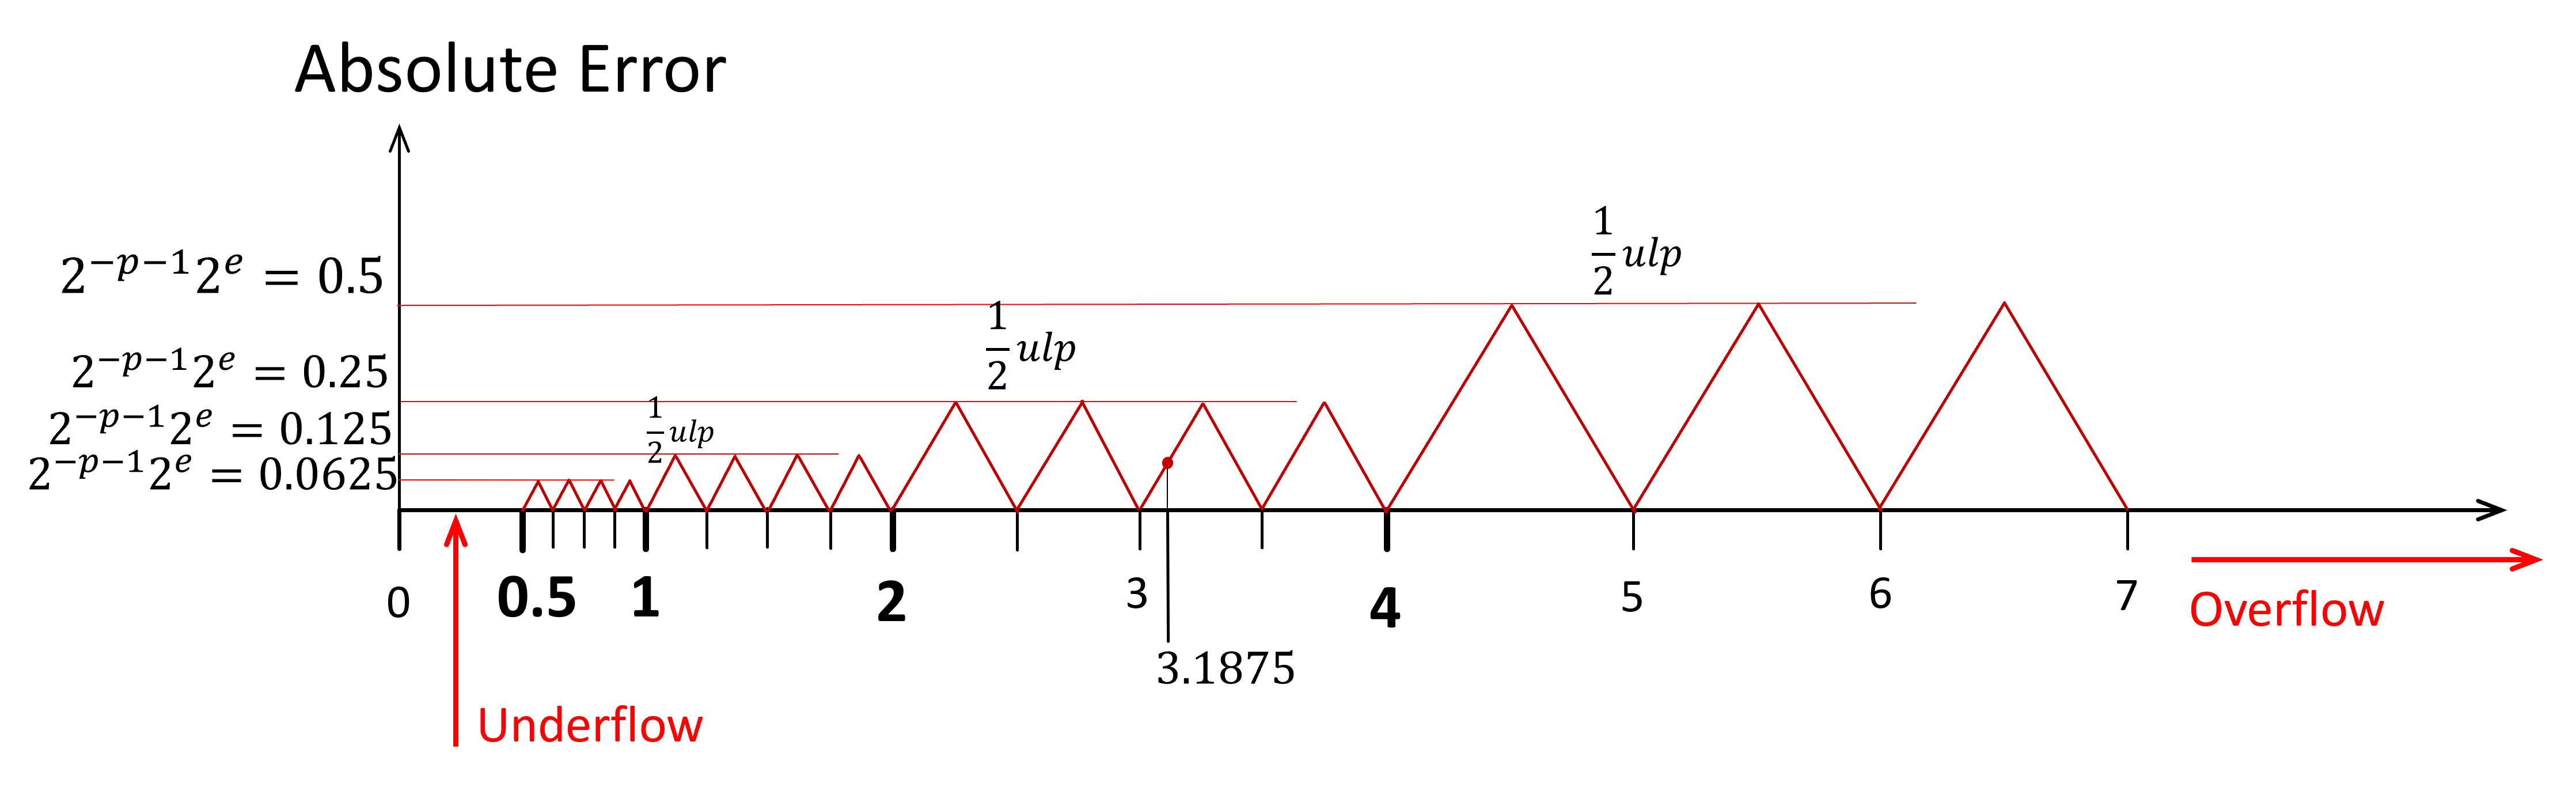
\includegraphics[width= \textwidth]{./doc/Figures/AbsErrorGraph.png}
%    \caption{Graphic of the absolute error committed when the real numbers are approximated by the nearest floating-point value with the 
%        maximum value represented for each window (exponent).}
%    \label{fig:AbsErrorGraph}
%\end{figure}
%
%\begin{figure}[h]
%    \centering
%    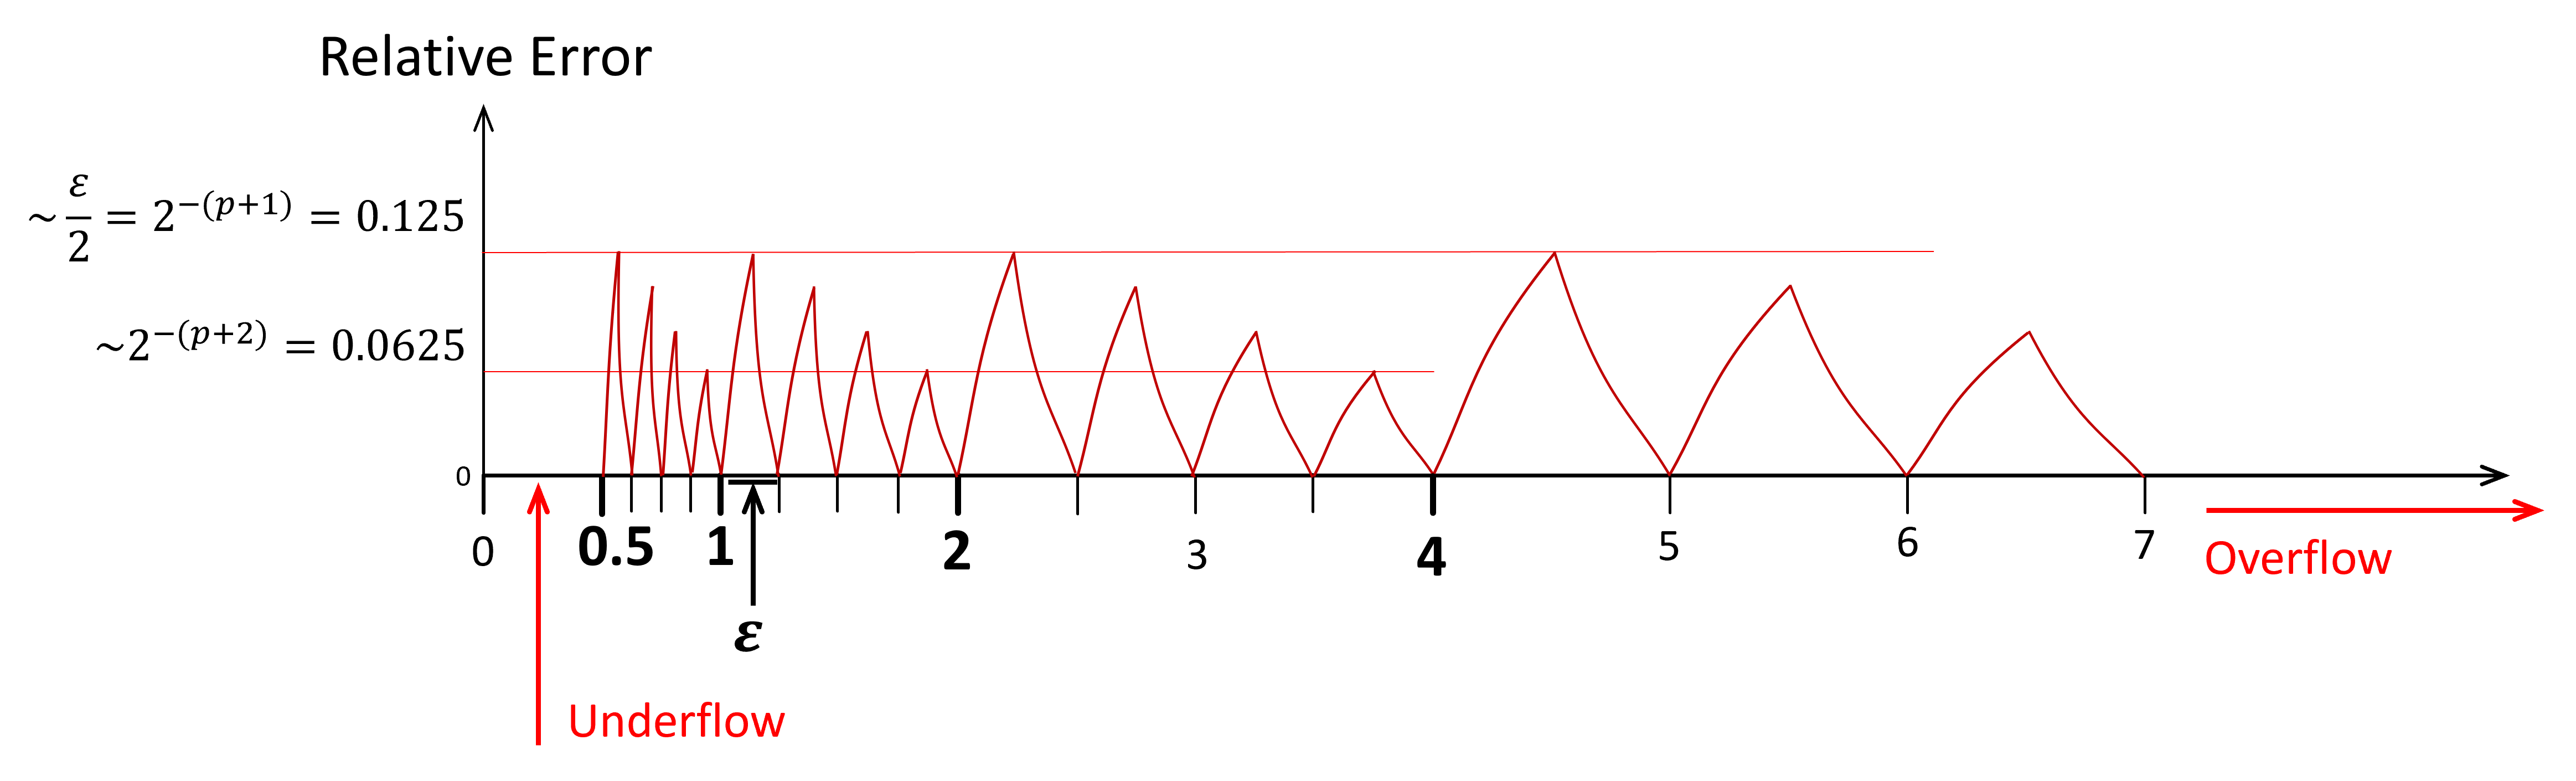
\includegraphics[width= \textwidth]{./doc/Figures/RelErrorGraph.png}
%    \caption{Graphic of the relative error committed when the real numbers are approximated by the nearest floating-point value with the 
%        maximum value represented for all windows (exponent).}
%    \label{fig:RelErrorGraph}
%\end{figure}
%
%\begin{IN}
%    The value $\frac{\beta}{2}\beta^{-p} = \epsilon$ is called machine epsilon, always take into account this magnitude because it bounds the 
%    relative error of any number when is rounded to the closest floating-point value. In the case of binary floating-point it can be 
%    expressed as $\epsilon = 2^{-p}$ taking the value of $2^{-24} \sim 5.96e-8$ in simple precision (23 bits plus 1 implicit bit), $2^{-53} 
%    \sim 1.11e-16$ in double precision and $2^{-113} \sim 9.63e-35$ in quadruple precision. In other conventions, the machine epsilon is 
%    considered the value $\beta^{1-p} = \epsilon$ which is the ulp for the value $1.0$ and in this case it is defined as: \textit{machine 
%        epsilon is defined as the difference between 1 and the next larger floating point number}.
%\end{IN}




    %--------------------------------------------------------------------------------------------------------------------------------------    
    \section{Decimal real number from its internal IEEE binary representation}


\FloatBarrier 
\begin{figure}[H]
    \centering
    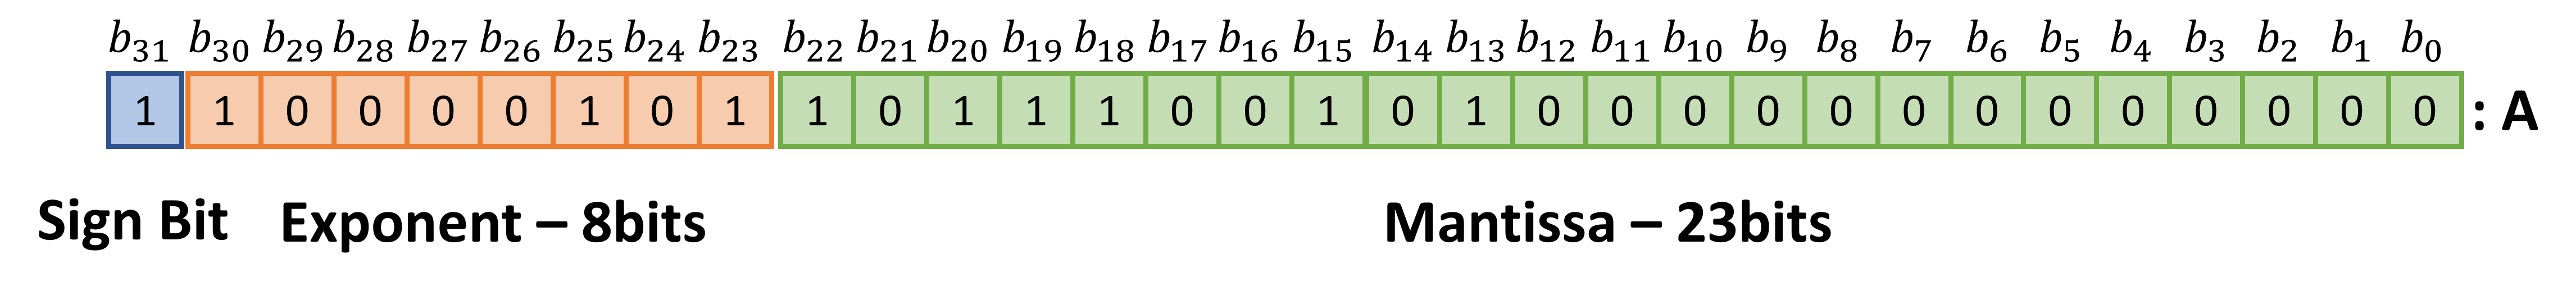
\includegraphics[width= \textwidth]{./doc/Figures/singlebits.png}
    \caption{Bit index for a single precision IEEE 754 floating-point (4 bytes).}
    \label{fig:singlebits}
\end{figure}

The decimal value for a single precision (\texttt{binary32}) floating point can be obtained trough the following expression (see Figure \ref{fig:singlebits}):
$$
   x = (-1)^{b_{31}}  \:  2^e  \: \left( 1 +   \sum_{i=1}^{23} b_{23-i} 2^{-i}    \right) 
$$
being $e$ the exponent already converted to decimal and properly biased. 
Notice that the implicit 1 is added to the sum which covers all the mantissa digits. 

The exponent uses a bias, also called  offset binary, to encode negative values $B = 2^{r-1} - 1 = 127$ ($r$ is the number of exponent digits). 
The following expression gives its decimal value:
$$
e = \sum_{j=0}^{7} b_{23+j} 2^j - B
$$
 

%The decimal value for a IEEE 754 floating-point value can be obtained trough the following expression (see Table \ref{tab:properties}):
%$$
%x = (-1)^{s}  2^e  \sum_{i=0}^{p} b_i 2^{-i} \quad \textnormal{with}\quad b_0 = 1
%$$
%being $s$ the sign bit, $e$ the exponent already converted to decimal and properly biased and $p$ the number of digits in the mantissa excluding the implicit 1. 
%Notice that $b_0 = 1$ considers the implicit 1 by adding $1\times2^0 = 1$ to the fractional mantissa.
% 
% The exponent uses a bias (or offset binary) to encode negative values. The following expression gives its decimal value:
% $$
% e = \sum_{j=0}^{r-1} b_j 2^j - \left( 2^{r-1} - 1 \right)
% $$
% being $r$ the number of exponent digits. 
 
\begin{IN}
    These expressions can be easily generalized by changing the bit index origins and upper limit of the sums:
    $$
    x = (-1)^{b_{p+r}}  2^e \left( 1 +   \sum_{i=1}^{p} b_{p-i} 2^{-i}    \right) 
    $$
    $$
    e = \sum_{j=0}^{r-1} b_{p+j} 2^j - B
    $$
    being $p$ the the number of digits in the mantissa (excluding the implicit 1), $r$ the number of exponent digits and $B = 2^{r-1} - 1$ (see Table \ref{tab:properties}).   
\end{IN}




 
 

%EJEMPLO
Now we can easily reconstruct the example in the Figure \ref{fig:ParametersIEEE}. Separating sign, exponent and mantissa we have the single precision binary: 

\texttt{1 10000101 10111001010000000000000}. 

The exponent is encoding the value:
$$
e = ( 2^0 + 2^1 + 2^7 ) - 127 = 6
$$
and the decimal value is:
$$
x = (-1)^1 \times 2^6 \times ( 1 + 2^{-1} + 2^{-3} + 2^{-4} + 2^{-5} + 2^{-8} + 2^{-10} ) = -110.3125_{10}
$$




%$$
%   \epsilon = m_1 2^e - m_2 2^e  = 2^{e-M} 
%$$
%Use scientific notation with ES format (normalized mantissa). 

    %--------------------------------------------------------------------------------------------------------------------------------------     
    \section{IEEE binary representation from decimal real numbers}

Let's revise the steps to encode a decimal number in IEEE 754 binary representation:

\begin{enumerate}
    \item Give a value to the sign bit: 1 for negative and 0 for positive.
    
    \item Convert the absolute value of your number to binary or similarly, to fixed-point representation. Right now there is not limit in the number of bits. 
      
    \item Move the binary point to the first position according to the binary scientific notation and then find the unbiased exponent.
    
    \item Omit the first 1, which will be implicit.
    
    \item Calculate the biased exponent by adding the bias $B = 2^{r-1}-1$ (check Table \ref{tab:properties}).
    
    \item Fill in the mantissa digits adding zeros at the right if necessary or truncating/rounding the excess of digits obtained in the conversion\footnote{The normal way to round the excess is by ``round to the nearest, ties to even''. If the (p+1)-th bit is a zero we chop the digits, if it is a 1 we add one to the p-th bit. The special case of a 1 in the (p+1)-th bit followed by zeros involves (similarly to the decimal system) that, if the p-th is a 1, we add one to the mantissa, if the p-th is a zero, we chop the digits.}.
\end{enumerate}




%EJEMPLO
Let's convert the number $-110.3125_{10}$ to a 32bits IEEE 754 floating point explaining step by step:

\begin{enumerate}
    \item This number is negative so the sign bit is a 1.
    
    \item The whole part is $110_{10}=\texttt{1101110}_2$ and the decimal part is $0.3125_{10}=\texttt{0.0101}_2$. Hence, the complete number in binary is:
    
     $\texttt{1101110.0101}_2$. 
    
    \item Moving the floating point: $\texttt{1101110.0101}=\texttt{1.1011100101} \times 2^6$.
    
    \item Omitting the implicit 1 we obtain the mantissa: 
    
    $\texttt{1.1011100101}\times2^6 \rightarrow \texttt{.1011100101}\times2^6$.
    
    \item To obtain the biased exponent we add $127$ since we are converting to single precision. Our exponent $6$ is covered by the value:
    
     $6 + 127 = 133_{10}= \texttt{10000101}_2$. 
    
    \item Writing the expressions for sign, exponent and mantissa and filling in the rest of mantissa digits with zeros at the right the result is: 
    
    $\texttt{1}\quad \texttt{10000101}\quad \texttt{10111001010000000000000}$
    
\end{enumerate}






    %-------------------------------------------------------------------------------------------------------------------------------------- 
    \FloatBarrier    
    \section{IEEE exceptions} \label{sec:exceptions}

The standard IEEE 754 reserves some combinations of binary digits for special situations: \texttt{NaN}, $\pm\infty$ or denormalised numbers (numbers in the gap that exits between the smallest normalised number representable (\texttt{tiny}) and the same negative value). In addition, take into account that there are two numbers equal to $0$: $\pm 0$ (see Table \ref{tab:SpecialValues}).

Infinity and NaN are essential to denote whether the result of a computation is too large to be represented in IEEE-754 (\textbf{overflow}) or a variable resulted in an illegal value (division $\frac{0}{0}$ for example). The operations between those special values are defined in the standard (see Table \ref{tab:SpecialOperations}).

The denormalised numbers (or subnormal numbers) are used when \textbf{underflow} occurs. Then, a gradual underflow is achieved so numbers too small to be represented (otherwise replaced by 0) are gradually decreased. From the representation point of view, the number is not treated with an implicit 1 before the binary point in the mantissa, but with a zero. Hence, the range of the mantissa is $\left[ 0, 1\right)$.


\begin{table}
    \centering
    \begin{tabular}{| c | c | l |}
        \hline
        Exponent & Mantissa & Value represented \\ \hline
        All 0's  & All 0's & $\pm 0 $ depending on the sign bit, they are equal  \\ \hline
        All 1's  & All 0's & $\pm \infty$ depending on the sign bit \\ \hline
        All 1's & NOT all 0's & Not a Number (\texttt{NaN})  \\ \hline
        All 0's  & NOT all 0's & Denormalised numbers  \\ \hline
    \end{tabular}
    \caption{Special binary combinations covered by the IEEE 754 standard.}
    \label{tab:SpecialValues}
\end{table}

\begin{table}
    \centering
    \begin{tabular}{| l | c |}
        \hline
        Operation & Result \\ \hline
        $ n / \left(\pm \infty\right) $            &     $	0$              \\ \hline
        $\pm \infty * \left( \pm \infty\right) $    &     $	\pm \infty$      \\ \hline
        $\pm$ nonZero$ / \pm 0 $            &    $	\pm \infty$       \\ \hline
        $\pm $finite$\quad * \pm \infty $      &    $	\pm \infty$       \\ \hline
        $\infty+\infty$  or  $\infty- \left(-\infty\right) $	     &       $+\infty$\\ \hline    
        $-\infty - \infty$   or  $-\infty + \left( -\infty \right) $   &        $	-\infty$\\ \hline
        $\pm 0 / \pm 0 $                  &        $	NaN$         \\ \hline
        $\pm \infty / \pm \infty $    &        $	NaN$     \\ \hline
        $\pm \infty * 0 $            &        $	NaN$     \\ \hline
        $ NaN == NaN $               &    $	False $      \\ \hline
    \end{tabular}
    \caption{Special operations covered by the IEEE 754 standard.}
    \label{tab:SpecialOperations}
\end{table}





    %--------------------------------------------------------------------------------------------------------------------------------------     
    \section{Declaring kind} 
    %\section{Practical guidance to use real numbers} 


Similarly to integers, a good practice is to write codes that can be used with different real precisions:
\texttt{kind=2, 4, 8}. To do that, do not specify the kind of any \textbf{variable}, just use \texttt{real :: x}. 
Then, the compiler assumes default real kind for all real variables. 
Generally, this default can be easily changed with a proper compilation option and then, 
the program does not depend on the precision imposed when it was written. 

The alternative is to explicitly declare the kind (precision) of any real variable: 
\begin{verbatim}
real(kind = 4) :: x1
real(kind = 8) :: x2
real(kind = 16) :: x3
\end{verbatim}

Instead of that, we propose to manage the compiler options and write with this notation:
\begin{verbatim}
    real :: x
\end{verbatim}

When declaring real \textbf{constants}, the situation is different. 
Consider for example the real constant \texttt{10.}. 
A specific kind type can be declared 
by underscoring the constant with its kind type or
by using exponential notation with \texttt{d} (double) or \texttt{q} (quadruple):

\newpage
\begin{verbatim}
10._4        
10._8    1d1     1.d1    1e1_8   1.e1_8
10._16   1q1     1.q1    1e1_16  1.e1_16
\end{verbatim}
However, this is not our recommended way to do it.

Consider not declaring the kind for any constant so it automatically adopts the default real kind value, use any of the following:
\begin{verbatim}
10.      1e1     1.e1    10e0   10E0    10.E0   10.e0
\end{verbatim}
First of all, notice that \texttt{10} can not be used since it would be treated as an integer. 
Secondly, remember that using exponential notation (\texttt{e} or \texttt{E}) does not automatically involves single precision. 
The \texttt{default real kind} compiler option rules its precision.

\begin{IN}
A program can be independent of declared precisions so the following compiler option rules the behaviour of all reals:

Default Real KIND: $\texttt{/real-size:{32\mid64\mid128}}$
\end{IN}






%RESTOS
%\begin{IN}
%    A program can be independent of declared precisions so the following compiler option rules the behaviour of all reals:
%    
%    Default Real KIND: $\texttt{/real-size:{32\mid64\mid128}}$
%    
%    Default Double Precision KIND: $\texttt{/double-size:{32\mid64\mid128}}$
%\end{IN}

%If the type of a variable is defined in the declaration of the variable it is typically used \texttt{real(kind = n) :: } or \texttt{real*n :: } where \texttt{n} is 4, 8 or 16. 
%Unless you have changed it, the default real kind is simple precision (\texttt{kind = 4}). 

%When declaring \textbf{constants}, the situation is different. 
%A specific kind type can be declared by underscoring the constant with its kind type:
%\begin{verbatim}
%    123.45_4
%    123.45_8
%    123.45_16
%\end{verbatim}
%However, this is not the common way to do it, 
%consider not declaring the kind for any constant neither so it automatically adopts the default real kind value.
%
%\textbf{Scientific notation} can also be used in languages like Fortran, for example, declaring the real constant $10.$ can be done equivalently in the following ways:
%\begin{verbatim}
%    10.
%    1e1
%    1.e1
%    10e0
%    10.E0
%    10.e0
%\end{verbatim}
%First of all, notice that \texttt{10} can not be used since it would be treated as an integer. 
%Secondly, remember that the kind of these constants \textbf{is not necessarily single precision}, default precision is being used with scientific notation so the \texttt{default real kind} option of the compiler rules the precision of these constants.
%
%Historically, if the scientific notation is mixed with the declaration of an specific kind, these declarations were used for double precision:
%\begin{verbatim}
%    1d1
%    1.d1
%    1e1_8
%    1.e1_8
%\end{verbatim}
%or for quadruple precision:
%\begin{verbatim}
%    1q1
%    1.q1
%    1e1_16
%    1.e1_16
%\end{verbatim}
%However, this is not our recommended way to do it, consider not declaring the kind for any constants so it automatically adopts the default real kind value.



    %--------------------------------------------------------------------------------------------------------------------------------------  
\newpage   
\section{\texttt{subroutine mantissa\_exponent\_base\_2}} 
The following subroutine allows to reconstruct a real number through its internal bits representation: 
%\vspace{0.5cm}
\listings{\home/IEEE_representation.f90}
{subroutine mantissa_exponent_base_2}{end subroutine}
{Subroutine to reconstruct the number in IEEE_representation.f90} 
This subroutine works by storing in a quadruple precision number any input value, 
either single, double or quadruple precision real. Then,  
the binary representation is written in a string called \texttt{bits}, 
the different parts are extracted (sign bit, exponent and mantissa) 
and the decimal value reconstructed. 
Notice the following: 
first, this code covers the normalized numbers and not the special values and denormalized numbers. 
Second, the conversion to quadruple precision carries with the round off error of the original precision and 
third, in order to write bits in the screen do not forget that leading zeros are not displayed.

Functions \texttt{normalized\_mantissa(string)} and \texttt{biased\_exponent(string)} returns the mantissa including an implicit 1 and the exponent biased with a bias value of 16383 from the input string of bits. 

\listings{\home/IEEE_representation.f90}
{function normalized_mantissa}{end function}
{normalized_mantissa function in IEEE_representation.f90} 

\listings{\home/IEEE_representation.f90}
{biased_exponent}{end function}
{biased_exponent function in IEEE_representation.f90} 

Call the program with the same real value declared as simple, double and quadruple precision and take a care look at the big differences in the reconstructed number, specially the significant digits for all the precisions. 







 






































%------------------------------------------------------------------------------------------------------------------------------------------------------
%------------------------------------------------------------------------------------------------------------------------------------------------------
%------------------------------------------------------------------------------------------------------------------------------------------------------
%------------------------------------------------------------------------------------------------------------------------------------------------------
%A FUTURO


%Poner ejemplos del epsilon en fortran
%Ver lo codigos que ya tengo hechos. Detalle de como mostrar resultados
%Recomendacion en la notacion


%Acabar el articulo de What Every... y capítulo de Trefethen


%
%This information can also be accessed by code, take a look at the useful intrinsic functions that can be used in Fortran.
%
%\begin{verbatim}
%    real(kind=4) :: x
%    real(kind=8) :: y
%    
%    write(*,*) 'Declaration of x with - real(kind = 4):: x'
%    write(*,*) 'Maximum value', huge(x)
%    write(*,*) 'Minimum value', tiny(x)
%    write(*,*) 'Round_off', epsilon(x)
%    write(*,*) 'Significant digits', precision(x)
%    
%    write(*,*) 'Declaration of y with - real(kind = 8) :: y'
%    write(*,*) 'Maximum value', huge(y)
%    write(*,*) 'Minimum value', tiny(y)
%    write(*,*) 'Round_off', epsilon(y)
%    write(*,*) 'Significant digits', precision(y)
%\end{verbatim}
%
%which results in:
%
%\begin{verbatim}
%    Declaration of x with - real(kind = 4):: x
%    Maximum value  3.4028235E+38
%    Minimum value  1.1754944E-38
%    Round_off  1.1920929E-07
%    Significant digits           6
%    
%    Declaration of y with - real(kind = 8) :: y
%    Maximum value  1.797693134862316E+308
%    Minimum value  2.225073858507201E-308
%    Round_off  2.220446049250313E-016
%    Significant digits          15
%\end{verbatim}



    %--------------------------------------------------------------------------------------------------------------------------------------
% \section{Operations}

%Take a look at the following example of simple arithmetic operations between different data types (whether different type or kind in the same type):
%
%\begin{verbatim} 
%    write(*,'(a20, f17.15)') '1.1/2.        ', 1.1/2. 
%    write(*,'(a20, f17.15)') '1.1e0/2e0     ', 1.1e0/2e0
%    write(*,'(a20, f17.15)') '1.1d0/2d0     ', 1.1d0/2d0 
%    
%    write(*,'(a20, f17.15)') '1.1/2         ', 1.1/2
%    
%    write(*,'(a20, f17.15)') '1.1/2d0       ', 1.1/2d0
%\end{verbatim}
%
%The result when the compiler has default real kind defined as simple precision is the following, try to understand why those results:
%
%\begin{verbatim}
%    1.1/2.        0.550000011920929 
%    1.1e0/2e0     0.550000011920929 
%    1.1d0/2d0     0.550000000000000 
%    
%    1.1/2         0.550000011920929 
%    
%    1.1/2d0       0.550000011920929 
%\end{verbatim}
%
%Let's analyse each example and obtain some conclusions from them. 
%
%The first three examples performs the same operation, it divides the number \texttt{1.1} (which does not have exact representation in the standard IEEE 754) by two, which is exact. They perform the operation with no precision imposed the first two of them and in double precision the third one. However, if we change the default real kind in the compiler options and impose to treat constants and variables as double precision by default, the result is:
%
%\begin{verbatim}
%    1.1/2.        0.550000000000000
%    1.1e0/2e0     0.550000000000000
%    1.1d0/2d0     0.550000000000000
%\end{verbatim}
%
%The conclusion to obtain from this is: write codes that do not depend on a precision, just use the first case (\texttt{1.1/2.}) and change the compiler options whether you need simple precision or double precision result. It is not necessary to write in each operation \texttt{d0} to make sure that the operation is performed in double precision, just configure the compiler to treat all constants (and variables) as double precision. In the next example it is demonstrated that writing (\textit{2.}) is not necessary neither. However, notice that in order to force the constant to be real (\texttt{e0}) is not needed. 
%
%Now take a look at the fourth example, it uses the integer 2 instead of converting it to a real number. While operations between two integer operands or between two real operands are developed as expected, a mixed-mode expression (where different data types are involved) must be treated with care. Arithmetic involving different types of operands or different kinds of the same type (i.e. \texttt{real (kind 4)} and \texttt{real (kind 8)}) will be carried out by converting the lowest-ranking operand to the highest-ranking operand so the result has this type and kind. The table \ref{tab:ranking} shows the ranking of each type. 
%
%\begin{table}[h]
%    \begin{tabular}{| c | c |}
%        
%        \hline
%        Data Type & Ranking \\ \hline
%        LOGICAL(1) and BYTE & Lowest \\ \hline
%        LOGICAL(2)     &  . \\ \hline
%        LOGICAL(4)     &  . \\ \hline
%        LOGICAL(8)      & . \\ \hline
%        INTEGER(1)     &  . \\ \hline
%        INTEGER(2)    &   . \\ \hline
%        INTEGER(4)    &   . \\ \hline
%        INTEGER(8)    &   . \\ \hline
%        REAL(4)     &  . \\ \hline
%        REAL(8)     &    .   \\ \hline
%        REAL(16)    &   . \\ \hline
%        COMPLEX(4)  &     . \\ \hline
%        COMPLEX(8)  &     . \\ \hline
%        COMPLEX(16) &    Highest\\ \hline
%        
%        
%    \end{tabular}                                                       
%    \caption{Ranking assigned to each data type, arithmetic will be performed with the highest ranking.}
%    \label{tab:ranking}
%\end{table}
%
%This means that the integer 2 is automatically converted to a real value (which has higher-ranking associated) and the operation is performed. If double precision is needed is simple, just change the compiler option and execute the same program:
%
%\begin{verbatim}
%    1.1/2         0.550000000000000
%\end{verbatim}
%
%The main conclusion is that there is no need of specifying always that constants are real values if the operation is performed with one operand being already real. But do not forget that at least one operand must define the type of operation to perform, if you do not write at least one real value, you are operating in the integers field and the divisions in the integer field totally ignore the decimal part of the result, so it is truncated (the rest of the operations in the integer field are performed as expected):
%
%\begin{verbatim}
%    write(*,'(a20, f17.15)') '1/3           ', 1/3
%\end{verbatim}
%
%which results in the :
%
%\begin{verbatim}
%    1/3           0.000000000000000
%\end{verbatim}
%
%The situation can be tricky when more operands are involved: 
%
%\begin{verbatim}
%    write(*,'(a20, f17.15)') '5/2 * 3. =      ', 5/2 * 3.
%    write(*,'(a20, f17.15)') '3. * 5/2 =      ', 3. * 5/2
%\end{verbatim}
%
%\begin{verbatim}
%    5/2 * 3. =      6.000000000000000
%    3. * 5/2 =      7.500000000000000
%\end{verbatim}
%
%Both are the same operation, however the first example is not properly performed since the precedence of the operation is from left to right in products and divisions. Hence, 5/2 is operated in first place, and the result is 2 in the integer field, which multiplied by 3. is 6. At least, in the division, it would be nice to force one value to be real with no need of changing the order of the operation. 
%
%Take a look at the following examples in real situations:
%PONER EJEMPLOS REALES
%%Ejemplo de dividir por 2. en grids
%%Otros ejemplos
%%Poner el caso de variable constante N que hay que pasar a real usando real(N) FUNDAMENTAL
%
%
%Finally, look at the fifth example, it can be a little tricky to understand at first. Notice that the compiler is configured for default real kind in simple precision so the value 1.1 is simple precision. According to the table above we could think that the value 1.1 is transformed to double precision in order to be operated with the value \texttt{2d0}. However, the result is clearly carrying with the round-off of the value 1.1 in simple precision. The reason is that the value 1.1 is stored in double precision but no transformed to double precision. 
%
%%Aqui poner los bits de este ejemplo
%
%If the same code is executed with default double precision then the value 1.1 is already double precision so there is not problem. Once again, according to our first conclusion, writing \texttt{2d0} in both cases is not necessary at all and just blurs the program.
%
%\begin{verbatim}
%    1.1/2d0       0.550000000000000
%\end{verbatim}
%
%%Profundizar en UNA sola operacion entre dos numeros, que precision asegura. epsilon y epsilon de la maquina
%
%
%
%
%To be explained:
%
%\begin{verbatim} 
%    x**2  = x * x 
%    
%    y = 2 * x 
%    
%    y = 2d0 * x 
%    
%    y = 2. * x 
%    
%    x**2d0 = exp( 2 * ln x ) 
%    
%    
%    x = 1 / 2
%    x = 1 / real(2) 
%    x = 1 / 2. 
%    
%    x = 1d0 * i / N  ! NO GUSTA 
%    
%    x = i / real(N) 
%    
%    ! same numbers 
%    x = 1 
%    x = 1. 
%    x = 1D0 
%    x = 1e0 
%    
%    y = x**2
%    y = x**2.
%    
%\end{verbatim} 






%------------------------------------------------------------------------------------------------------------------------------------------------------
%------------------------------------------------------------------------------------------------------------------------------------------------------
%------------------------------------------------------------------------------------------------------------------------------------------------------
%------------------------------------------------------------------------------------------------------------------------------------------------------
%RESTOS


%\newpage
%\begin{table}[H]
%    \begin{flushright}
%        \begin{turn}{90}
%            \begin{tabular}{| r | c | c | c | c | c | c | c | c |}
%                
%                \hline
%                Name & Sign & Exp. & Mantissa & Exp. Bias & Bits precision & \begin{tabular}{@{}c@{}}Normalized \\ range \end{tabular}   & Approximate decimal  & Precision \\ \hline
%                
%                \begin{tabular}{@{}c@{}}Single precision \\ (binary32) \end{tabular}      & 1 & 8  & 23    & +127   & 24 & \begin{tabular}{@{}c@{}}$\pm2^{−126}$ to \\$\pm2^{127+1}$  \end{tabular}    & \begin{tabular}{@{}c@{}}$\pm1.18\cdot10^{ −38}$ to \\ $\pm3.4\cdot10^{38}$ \end{tabular}     & \sim 7.2 digits  \\ \hline
%                
%                \begin{tabular}{@{}c@{}}Double precision \\ (binary64) \end{tabular}    & 1 & 11 & 52    & +1023  & 53 & \begin{tabular}{@{}c@{}}  $\pm2^{−1022}$ to\\  $\pm2^{1023+1}$\end{tabular}  & \begin{tabular}{@{}c@{}} $\pm2.23\cdot10^{ −308}$ to \\ $\pm1.80\cdot10^{308}$ \end{tabular} & \sim 15.9 digits        \\  \hline
%                
%                \begin{tabular}{@{}c@{}} Quadruple precision\\(binary128) \end{tabular}   & 1 & 15 & 112   & +16383 & 113 & \begin{tabular}{@{}c@{}}  $\pm2^{-16382}$ to\\  $\pm2^{16383+1}$\end{tabular}   & \begin{tabular}{@{}c@{}} $\pm3.3621\cdot 10^{-4932}$ to \\ $\pm1.1897\cdot10^{4932}$ \end{tabular}  & \sim 19.2 digits          \\ \hline
%                
%            \end{tabular}                                                       
%        \end{turn}
%        \caption{Main properties of the different precisions covered by the IEEE 754 standard.}
%        \label{tab:properties}
%    \end{flushright}
%\end{table}

%\newpage
%\begin{table}[H]
%    \begin{flushleft}
%        \begin{turn}{90}
%            \begin{tabular}{| r | c | c | c | c | c |}
%                
%                \hline
%                Name & Sign bits & Exp.bits & Mantissa bits & Exp. Bias & Bits precision \\ \hline
%                
%                \begin{tabular}{@{}c@{}}Single precision \\ (binary32) \end{tabular}      & 1 & 8  & 23    & +127   & 24  \\ \hline
%                
%                \begin{tabular}{@{}c@{}}Double precision \\ (binary64) \end{tabular}    & 1 & 11 & 52    & +1023  &   53  \\  \hline
%                
%                \begin{tabular}{@{}c@{}} Quadruple precision\\(binary128) \end{tabular}   & 1 & 15 & 112   & +16383 & 113 \\ \hline
%                
%            \end{tabular}                                                       
%        \end{turn}
%        \caption{Fruta disponible}
%        \label{tab:properties}
%    \end{flushleft}
%\end{table}
%\begin{table}[H]
%    \begin{flushright}
%        \begin{turn}{90}
%            \begin{tabular}{| r | c | c | c |}
%                
%                \hline
%                Name & \begin{tabular}{@{}c@{}}Normalized \\ range \end{tabular}   & Approximate decimal  & Precision \\ \hline
%                
%                \begin{tabular}{@{}c@{}}Single precision \\ (binary32) \end{tabular}      &  \begin{tabular}{@{}c@{}}$\pm2^{−126}$ to \\$\pm2^{127+1}$  \end{tabular}    & \begin{tabular}{@{}c@{}}$\pm1.18\cdot10^{ −38}$ to \\ $\pm3.4\cdot10^{38}$ \end{tabular}     & \sim 7.2 digits  \\ \hline
%                
%                \begin{tabular}{@{}c@{}}Double precision \\ (binary64) \end{tabular}    &  \begin{tabular}{@{}c@{}}  $\pm2^{−1022}$ to\\  $\pm2^{1023+1}$\end{tabular}  & \begin{tabular}{@{}c@{}} $\pm2.23\cdot10^{ −308}$ to \\ $\pm1.80\cdot10^{308}$ \end{tabular} & \sim 15.9 digits        \\  \hline
%                
%                \begin{tabular}{@{}c@{}} Quadruple precision\\(binary128) \end{tabular}   & \begin{tabular}{@{}c@{}}  $\pm2^{-16382}$ to\\  $\pm2^{16383+1}$\end{tabular}   & \begin{tabular}{@{}c@{}} $\pm3.3621\cdot 10^{-4932}$ to \\ $\pm1.1897\cdot10^{4932}$ \end{tabular}  & \sim 19.2 digits          \\ \hline
%                
%            \end{tabular}                                                       
%        \end{turn}
%        \caption{Fruta disponible}
%        \label{tab:properties}
%    \end{flushright}
%\end{table}



